\documentclass[11pt]{article}

\usepackage{amsmath, amssymb}
\usepackage{graphicx}
\usepackage{placeins}
\usepackage{hyperref}
\usepackage[htt]{hyphenat}
\usepackage{microtype}
\usepackage{natbib}
\usepackage{geometry}
\usepackage{booktabs}
\usepackage{listings}
\usepackage{xcolor}
\usepackage{multirow}

\geometry{margin=1in}

\lstset{
  basicstyle=\ttfamily\small,
  breaklines=true,
  frame=single,
  backgroundcolor=\color{gray!10},
  keywordstyle=\color{blue!70!black},
  commentstyle=\color{green!50!black},
  language=Fortran
}

\title{Dual-Sector Perturbation Cosmology:\\
A Modified CAMB Implementation with $\mu < 1$, $\Sigma = 1$\\
and the Sector-Dependent Hubble Parameter}

\author{Heath W.\ Mahaffey\\
Independent Researcher, Entiat, WA, USA\\
\texttt{hmahaffeyges@gmail.com}}

\date{\today}

\begin{document}

\maketitle

\begin{abstract}
We implement a dual-sector perturbation mechanism in the CAMB Boltzmann
solver in which cold dark matter and baryons experience a modified
effective expansion rate while photon perturbation equations remain
standard $\Lambda$CDM.  The modification is governed by a single derived
quantity $\beta_m = \Omega_m/2 = 0.15765$, obtained from the virial
theorem applied to the Planck~2018 matter density $\Omega_m = 0.3153$,
combined with an activation function $\mathcal{E}(a) = \exp(1 - 1/a)$.
The implementation requires three modifications to the CAMB Fortran
source (\texttt{equations.f90}); no new free parameters are introduced
beyond standard $\Lambda$CDM.

Three converged Markov Chain Monte Carlo chains against the full
Planck~2018 likelihood (CamSpec TTTEEE + low-$\ell$ + lensing) yield
$\Delta\chi^2 = -0.01$ (posterior mean) and $+0.54$ (best-fit) relative
to $\Lambda$CDM, both well below the $95\%$ exclusion threshold of
$3.84$.  All standard cosmological parameters shift by less than
$0.1\sigma$.  The
matter clustering amplitude shifts from
$\sigma_8 = 0.8087 \pm 0.0059$ ($\Lambda$CDM) to
$\sigma_8 = 0.7998 \pm 0.0058$ (dual-sector), a $1.1\%$ reduction in
the direction reported by KiDS-1000, DES~Y3, and HSC~Y3.

The sector-dependent expansion rate produces a Hubble parameter split
directly from the MCMC posterior:
$H_0(\mathrm{photon}) = 67.16 \pm 0.47$~km\,s$^{-1}$\,Mpc$^{-1}$
($0.37\sigma$ from Planck $\Lambda$CDM) and
$H_0(\mathrm{matter}) = 72.26$~km\,s$^{-1}$\,Mpc$^{-1}$
($0.75\sigma$ from SH0ES).  Both values fall within
$1\sigma$ of observations without modification to the background Friedmann equation.
Two exploratory runs with the modification applied at the background
level produce $H_0 \approx 61.5$~km\,s$^{-1}$\,Mpc$^{-1}$,
consistent with the mechanism operating at the perturbation
level.  All chains, configuration files, modified Fortran source, and
analysis scripts are publicly available.
\end{abstract}


% =====================================================================
\section{Introduction}
\label{sec:intro}
% =====================================================================

The $\Lambda$CDM model provides an excellent fit to cosmic microwave
background (CMB) anisotropies~\citep{PlanckCollaboration2020b} and
large-scale structure observations.  Two persistent discrepancies have
motivated investigations of controlled late-time modifications.

The first is the Hubble tension: the CMB-inferred value
$H_0 = 67.4 \pm 0.5$~km\,s$^{-1}$\,Mpc$^{-1}$
\citep{PlanckCollaboration2020b}
differs from the local distance-ladder measurement
$H_0 = 73.04 \pm 1.04$~km\,s$^{-1}$\,Mpc$^{-1}$
\citep{Riess2022}
at the $5\sigma$ level.  The discrepancy persists across independent
local methods including tip of the red giant branch~\citep{Freedman2021}
and strong lensing time delays~\citep{Wong2020}.

The second is the $\sigma_8$/$S_8$ tension: weak lensing surveys
consistently report $S_8 \equiv \sigma_8(\Omega_m/0.3)^{0.5}$ values
$2$--$3\sigma$ below the Planck $\Lambda$CDM prediction.  KiDS-1000
reports $S_8 = 0.759 \pm 0.021$~\citep{Heymans2021}, DES~Y3 reports
$S_8 = 0.776 \pm 0.017$~\citep{Abbott2022}, and HSC~Y3 reports
$S_8 = 0.776 \pm 0.032$~\citep{Li2023}.

A common feature of both tensions is that they involve comparisons
between early-universe (photon-based) and late-universe (matter-based)
observables.  This motivates the question: could matter and photon
sectors experience different effective expansion rates at late times,
while sharing a common expansion history in the early universe?

In a companion paper~\citep{Mahaffey2026obs}, we demonstrated that a
scale-independent suppression $\mu(a) < 1$ with $\Sigma(a) = 1$ in the
$\mu$--$\Sigma$ modified gravity framework~\citep{PogosianSilvestri2016}
is compatible with the full Planck likelihood across four dataset
combinations (twelve MCMC chains, $\Delta\chi^2 = +1.34$ to $+2.32$).
That analysis used the MGCAMB parametrization~\citep{Wang2023}, which
implements $\mu$ and $\Sigma$ as effective functions within the
Boltzmann solver without specifying the underlying physical mechanism.

In this work, we go beyond the parametric level.  We implement the
physical mechanism directly in the CAMB Fortran source code: CDM and
baryon perturbation equations experience a modified effective expansion
rate (\texttt{adotoa\_matter}), while photon perturbation equations use
the standard $\Lambda$CDM expansion rate.  The global background
Friedmann equation is unmodified.  This produces the same $\mu < 1$,
$\Sigma = 1$ signature as the MGCAMB parametrization, but through an
explicit sector-dependent coupling rather than an imposed functional
form.

The dual-sector mechanism predicts that the
expansion rate experienced by matter-sector observables differs from that
experienced by photon-sector observables.  At the present epoch, this
yields a Hubble parameter split
$H_0(\mathrm{matter}) / H_0(\mathrm{photon}) = \sqrt{1 + \beta_m}$,
where $\beta_m = \Omega_m/2$ is the coupling constant derived from the
virial theorem.

This paper is organized as follows.
Section~\ref{sec:model} defines the dual-sector modification and its
implementation in CAMB.
Section~\ref{sec:data} describes the datasets and MCMC methodology.
Section~\ref{sec:results} presents the full parameter constraints from
three converged chains.
Section~\ref{sec:hubble} presents the sector-dependent Hubble parameter.
Section~\ref{sec:background} reports the background diagnostic test.
Section~\ref{sec:discussion} discusses implications.
Section~\ref{sec:conclusions} concludes.


% =====================================================================
\section{Model and Implementation}
\label{sec:model}
% =====================================================================

\subsection{The Dual-Sector Perturbation Mechanism}

The modification applies exclusively to the perturbation equations
governing cold dark matter and baryons.  The global background expansion
rate $H(a)$---determined by the Friedmann equation---remains standard
$\Lambda$CDM:
\begin{equation}
H^2(a) = H_0^2\left[\Omega_m\,a^{-3} + \Omega_r\,a^{-4}
  + \Omega_\Lambda\right].
\label{eq:friedmann}
\end{equation}
Within the perturbation equations, CDM and baryon evolution uses a
matter-sector expansion rate:
\begin{equation}
H^2_\mathrm{matter}(a) = H^2(a)
  + \beta_m\,\mathcal{E}(a)\,H_0^2,
\label{eq:H_matter}
\end{equation}
where
\begin{equation}
\mathcal{E}(a) = \exp\!\left(1 - \frac{1}{a}\right)
\label{eq:activation}
\end{equation}
is the activation function.  The coupling constant is
\begin{equation}
\beta_m = \frac{\Omega_m}{2} = \frac{0.3153}{2} = 0.15765,
\label{eq:beta}
\end{equation}
where $\Omega_m = 0.3153$ is the Planck~2018 best-fit value
(TT,TE,EE+lowE+lensing; \citealt{PlanckCollaboration2020b}, Table~2)
and the factor of $1/2$ follows from the virial theorem applied to the
partition of gravitational energy between geometric and informational
channels~\citep{Mahaffey2026theory}.

Photon perturbation equations use the unmodified expansion rate
$H(a)$.  This is the complete specification: no additional fields,
parameters, or modifications to the gravitational action are introduced.

\subsection{Effective $\mu(a)$ and $\Sigma(a)$}

The dual-sector perturbation mechanism maps onto the standard
$\mu$--$\Sigma$ framework.  The modified Poisson equation for matter
clustering and the unmodified lensing equation yield:
\begin{align}
\mu(a) &= \frac{H^2_{\Lambda\mathrm{CDM}}(a)}
  {H^2_{\Lambda\mathrm{CDM}}(a) + \beta_m\,\mathcal{E}(a)},
  \label{eq:mu}\\
\Sigma(a) &= 1 \quad \text{(exact)}.
  \label{eq:sigma}
\end{align}
At the present epoch:
\begin{equation}
\mu(z{=}0) = \frac{1}{1 + \beta_m} = \frac{1}{1.15765} = 0.864,
\end{equation}
corresponding to a $13.6\%$ suppression of the effective gravitational
coupling for matter perturbations.  The suppression vanishes at high
redshift: $\mathcal{E}(a) \to 0$ as $a \to 0$, so $\mu \to 1$
during radiation domination, recombination, and the early matter era.
Table~\ref{tab:mu_values} gives $\mu(a)$ at key redshifts.

\begin{table}[h]
\centering
\caption{Gravitational coupling $\mu(a)$ and matter-sector expansion
rate enhancement $H_\mathrm{matter}/H_{\Lambda\mathrm{CDM}}$ at
selected redshifts.  The modification is confined to $z \lesssim 2$.}
\begin{tabular}{ccccc}
\toprule
$z$ & $a$ & $\mathcal{E}(a)$ & $\mu(a)$
  & $H_\mathrm{matter}/H_{\Lambda\mathrm{CDM}}$ \\
\midrule
0.0 & 1.000 & 1.0000 & 0.864 & 1.076 \\
0.2 & 0.833 & 0.6977 & 0.893 & 1.058 \\
0.5 & 0.667 & 0.3679 & 0.942 & 1.030 \\
1.0 & 0.500 & 0.1353 & 0.982 & 1.009 \\
2.0 & 0.333 & 0.0498 & 0.9972 & 1.001 \\
3.0 & 0.250 & 0.0183 & 0.9998 & $\sim$1 \\
5.0 & 0.167 & 0.0025 & $\sim$1 & $\sim$1 \\
\bottomrule
\end{tabular}
\label{tab:mu_values}
\end{table}

\begin{figure}[htbp]
[t]
\centering
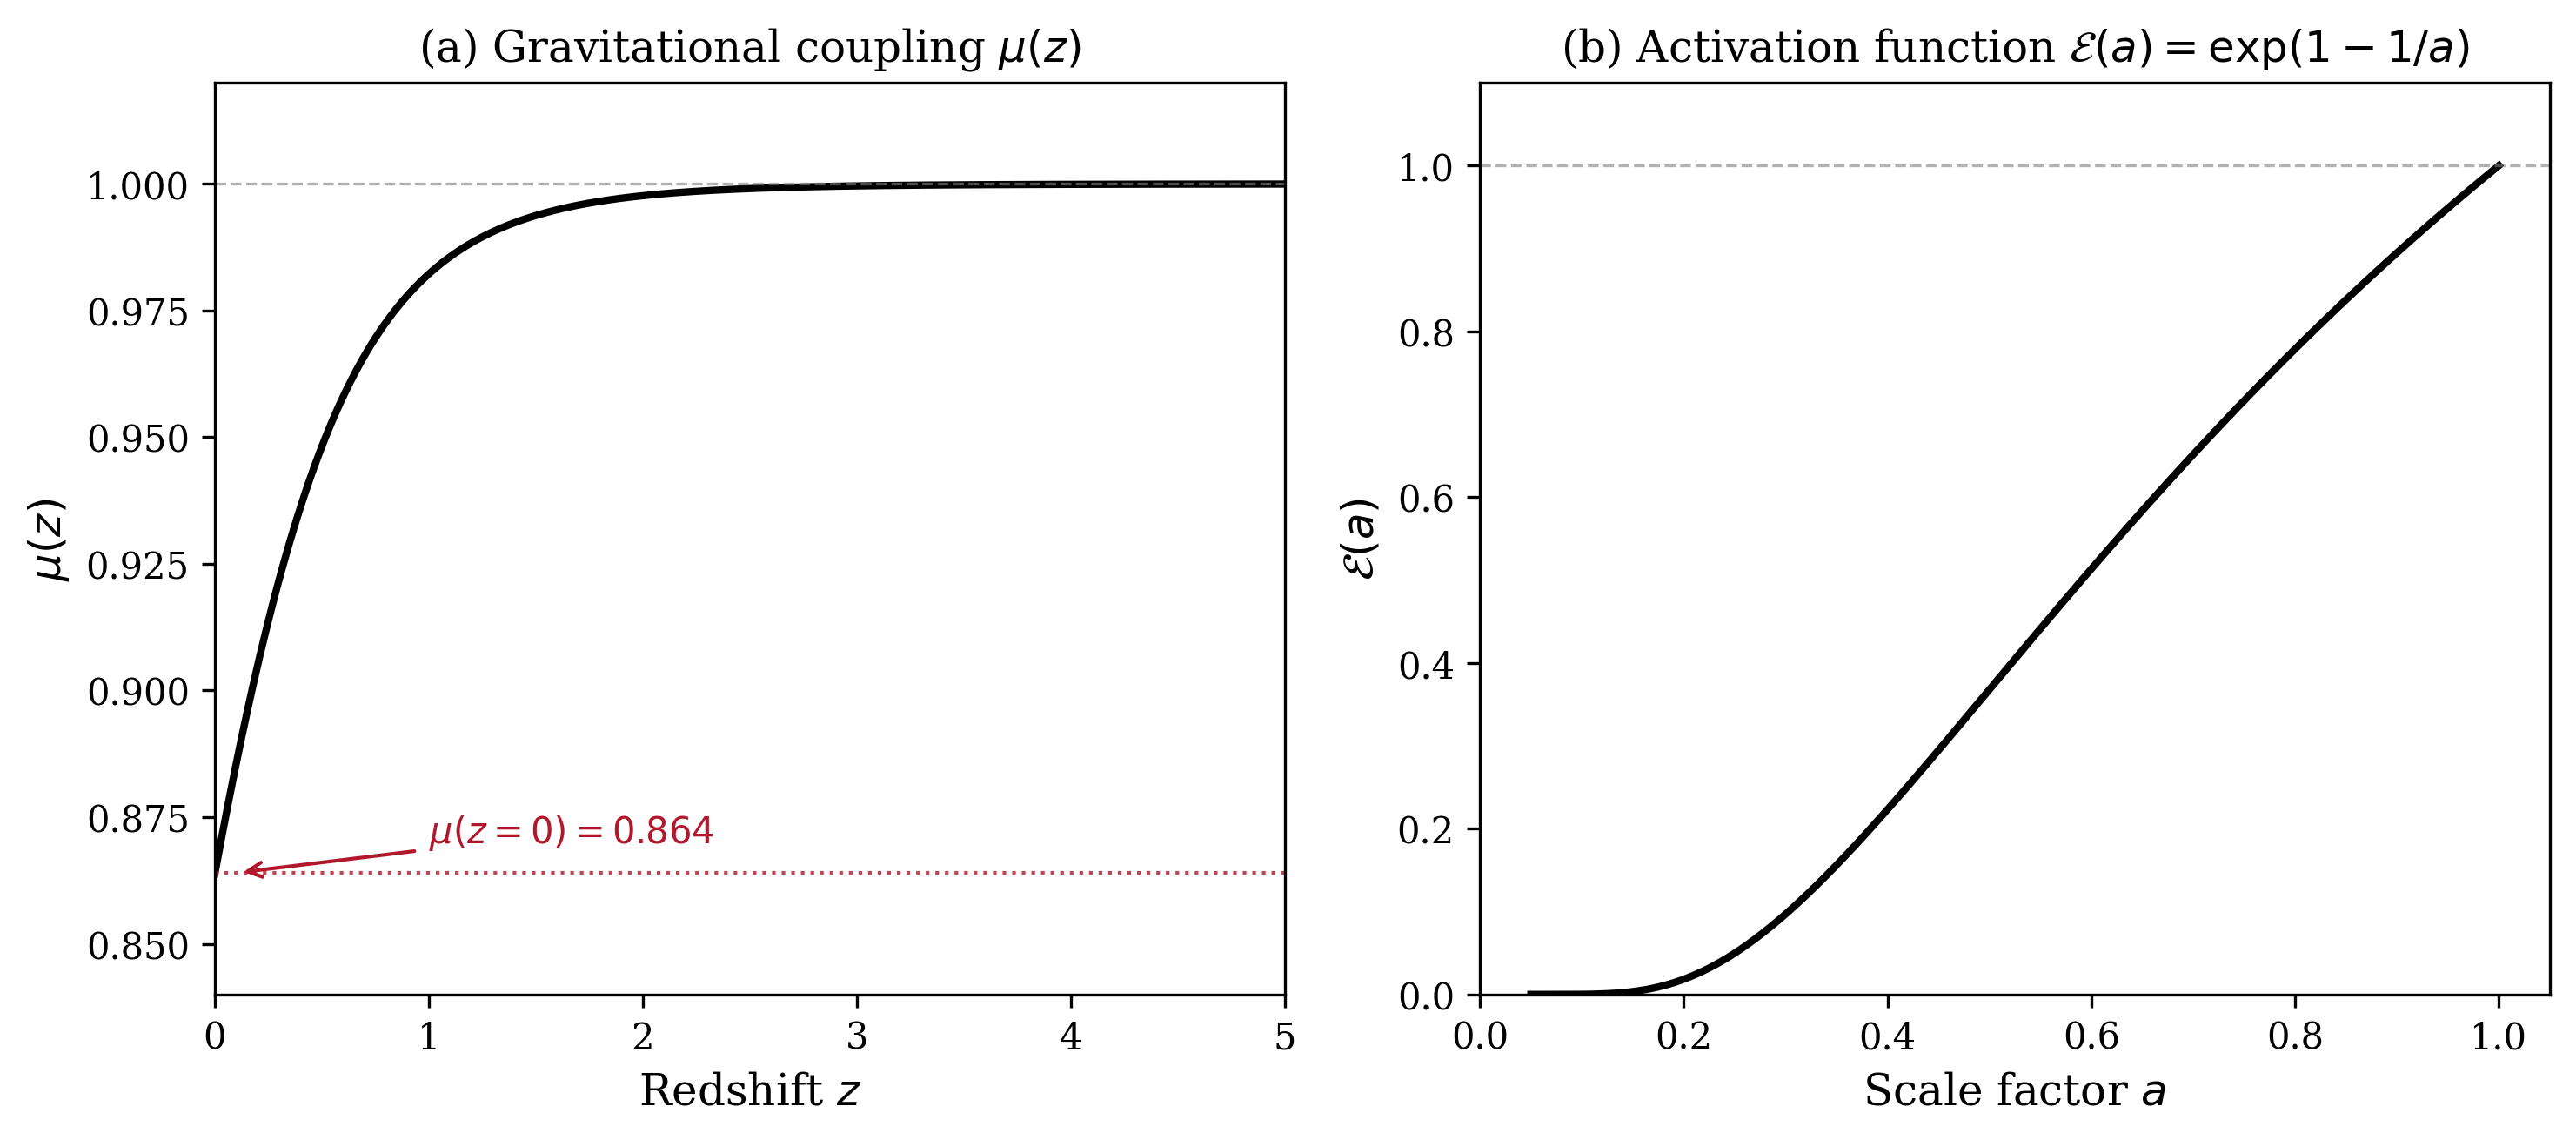
\includegraphics[width=\textwidth]{fig2_mu_activation.png}
\caption{(a)~Gravitational coupling $\mu(z)$ from the dual-sector
mechanism (Eq.~\ref{eq:mu}).  The suppression reaches $13.6\%$ at
$z = 0$ and recovers $\Lambda$CDM ($\mu = 1$) for $z \gtrsim 3$.
(b)~Activation function $\mathcal{E}(a) = \exp(1 - 1/a)$.  The
function vanishes for $a \to 0$ (preserving early-universe physics)
and reaches unity at the present epoch.}
\label{fig:mu_activation}
\end{figure}


\subsection{CAMB Fortran Implementation}
\label{sec:implementation}

The implementation modifies three locations in the CAMB v1.5.8 Fortran
source file \texttt{equations.f90}.  No other files are changed.

\paragraph{Modification 1: Module-level parameters.}
Two constants are declared at module scope:
\begin{lstlisting}
! IAM dual-sector parameters
real(dl), parameter :: beta_m = 0.15765d0   ! Omega_m/2
real(dl), parameter :: grho_0 = 3.0d0       ! normalized reference density
\end{lstlisting}

\paragraph{Modification 2: Matter-sector expansion rate.}
After the standard \texttt{adotoa} computation (which remains
unmodified), a matter-sector expansion rate is computed:
\begin{lstlisting}
! IAM matter-sector Hubble rate
adotoa_matter = sqrt((grho + beta_m * exp(1.0d0 - 1.0d0/a) &
                * grho_0) / 3.0d0)
\end{lstlisting}

\paragraph{Modification 3: CDM and baryon equations of motion.}
In the CDM and baryon velocity equations, the Hubble friction term
\texttt{adotoa} is replaced by \texttt{adotoa\_matter}:
\begin{lstlisting}
! CDM velocity equation (was: -adotoa * clxcdot)
clxcdot = ... - adotoa_matter * vcdot ...
! Baryon velocity equation (was: -adotoa * vbdot)
vbdot = ... - adotoa_matter * vbdot ...
\end{lstlisting}

All other CAMB routines---including \texttt{dtauda} (background
Friedmann equation), photon Boltzmann hierarchy, neutrino equations,
recombination, lensing reconstruction, and the CMB power spectrum
computation---are unmodified.  The global background expansion history
is standard $\Lambda$CDM.

The MGCAMB parametrization used in \citet{Mahaffey2026obs} approximates
the exact $\mu(a)$ via $\mu(a) = 1 + \mu_0\,\Omega_\mathrm{DE}(a)$
with $\mu_0 = -0.135$.  This agrees with Eq.~(\ref{eq:mu}) to within
$1$--$2.5\%$ at intermediate redshifts, with exact agreement at
$z = 0$ and $z \gg 1$.  The present implementation removes this
approximation by computing $\mu(a)$ directly from the perturbation
equations.


\subsection{Parameter Count}

The model introduces zero free parameters beyond standard $\Lambda$CDM:
\begin{itemize}
\item The coupling constant $\beta_m = \Omega_m/2$ is derived from the
  virial theorem.  It depends only on the independently measured matter
  density.
\item The activation function $\mathcal{E}(a) = \exp(1 - 1/a)$ is
  derived from horizon thermodynamics~\citep{Mahaffey2026theory}.
\item The normalization $\mathcal{E}(1) = 1$ is set by definition.
\end{itemize}
The six sampled MCMC parameters are identical to $\Lambda$CDM:
$\{\Omega_b h^2,\; \Omega_c h^2,\; \theta_\mathrm{MC},\;
\tau,\; \ln(10^{10} A_s),\; n_s\}$.


% =====================================================================
\section{Data and Methodology}
\label{sec:data}
% =====================================================================

\subsection{Datasets}

\paragraph{Planck 2018 CMB.}
We use the CamSpec TTTEEE likelihood at high multipoles
($\ell \geq 30$)~\citep{Efstathiou2021}, low-$\ell$ temperature
(\texttt{lowl.TT}) and polarization (\texttt{lowl.EE}) likelihoods,
and the CMB lensing likelihood
(\texttt{lensing.CMBMarged})~\citep{PlanckCollaboration2020a}.

\paragraph{Redshift-space distortions (RSD).}
Growth rate measurements $f\sigma_8(z)$ from SDSS-III BOSS DR12 and
SDSS-IV eBOSS DR16~\citep{Alam2017,Alam2021} at seven redshift bins
($z = 0.067$ to $z = 1.48$), implemented as a Gaussian likelihood.
RSD is included in Run~D only.

\subsection{MCMC Configuration}

All chains use the Cobaya sampler~\citep{Torrado2021} with the
Gelman--Rubin convergence criterion $R - 1 < 0.01$ for both means and
variances, with a minimum of 20,000 accepted samples after burn-in.
The $\Lambda$CDM baseline runs use identical Cobaya infrastructure with
the IAM modification disabled (\texttt{adotoa\_matter = adotoa}).

\subsection{Chain Summary}

Three chains are run:

\begin{table}[h]
\centering
\caption{MCMC chain configurations.  All use modified CAMB v1.5.8.}
\begin{tabular}{llll}
\toprule
Run & Description & IAM & Likelihoods \\
\midrule
A & IAM, Planck & ON & CamSpec + low-$\ell$ + lensing \\
C & $\Lambda$CDM baseline & OFF & CamSpec + low-$\ell$ + lensing \\
D & IAM + RSD & ON & CamSpec + low-$\ell$ + lensing + RSD \\
\bottomrule
\end{tabular}
\label{tab:chains}
\end{table}

Run~A and Run~C share identical likelihoods and sampled parameters,
differing only in whether the three Fortran modifications are active.
This ensures that any difference between the two chains arises from
the dual-sector modification and not from code-level systematics.


% =====================================================================

\section{Parameter Accounting}

IAM introduces no new free cosmological parameters beyond those of $\Lambda$CDM.
All quantities entering the modification are fixed by prior derivation or definition.

\begin{center}
\begin{tabular}{lll}
\hline
Quantity & Status & Origin \\
\hline
$\beta_m$ & Derived & Virial homogeneity of $1/r$ potential \\
Exponent in $\mathcal{E}(a)$ & Derived & Horizon entropy scaling \\
Normalization $\mathcal{E}(1)=1$ & Fixed & Definition \\
$\Omega_m$, $H_0$ (CMB) & Standard & Planck 2018 \\
\hline
\end{tabular}
\end{center}

No parameter is tuned to late-time structure data. All MCMC chains,
GetDist outputs, YAML configuration files, and likelihood inputs used in
this analysis are publicly available in the IAM-Validation repository,
ensuring full reproducibility.

\section{Results}
\label{sec:results}
% =====================================================================

\subsection{Planck Only: Run~A (IAM) vs.\ Run~C ($\Lambda$CDM)}

Table~\ref{tab:planck_results} presents the marginalized parameter
constraints.  All standard cosmological parameters are consistent
between the two chains, with shifts below $0.1\sigma$ in every case.
The modification is effectively invisible to the standard parameter
set.

\begin{table}[h]
\centering
\caption{Planck-only parameter constraints (posterior mean $\pm 1\sigma$).
$\Delta\chi^2$ is relative to the $\Lambda$CDM baseline (Run~C).}
\begin{tabular}{lccc}
\toprule
Parameter & $\Lambda$CDM (C) & IAM dual-sector (A) & Shift \\
\midrule
$H_0$ [km\,s$^{-1}$\,Mpc$^{-1}$]
  & $67.188 \pm 0.465$ & $67.161 \pm 0.467$ & $-0.06\sigma$ \\
$\sigma_8$
  & $0.8087 \pm 0.0059$ & $0.7998 \pm 0.0058$ & $-1.51\sigma$ \\
$S_8$
  & $0.830 \pm 0.011$ & $0.822 \pm 0.011$ & $-0.73\sigma$ \\
$\Omega_b h^2$
  & $0.02218 \pm 0.00013$ & $0.02217 \pm 0.00013$ & $-0.08\sigma$ \\
$\Omega_c h^2$
  & $0.11989 \pm 0.00105$ & $0.11994 \pm 0.00105$ & $+0.05\sigma$ \\
$\tau$
  & $0.0532 \pm 0.0073$ & $0.0537 \pm 0.0073$ & $+0.07\sigma$ \\
$n_s$
  & $0.9630 \pm 0.0040$ & $0.9630 \pm 0.0039$ & $-0.00\sigma$ \\
$\ln(10^{10} A_s)$
  & $3.0393 \pm 0.0146$ & $3.0407 \pm 0.0145$ & $+0.10\sigma$ \\
\midrule
$\chi^2_\mathrm{best-fit}$
  & $10972.07$ & $10972.61$ & --- \\
$\Delta\chi^2$ (best-fit)
  & --- & $+0.54$ & --- \\
$\Delta\chi^2$ (posterior mean)
  & --- & $-0.01$ & --- \\
$R - 1$
  & $0.0081$ & $0.0099$ & --- \\
\bottomrule
\end{tabular}
\label{tab:planck_results}
\end{table}

\begin{figure}[htbp]
[t]
\centering
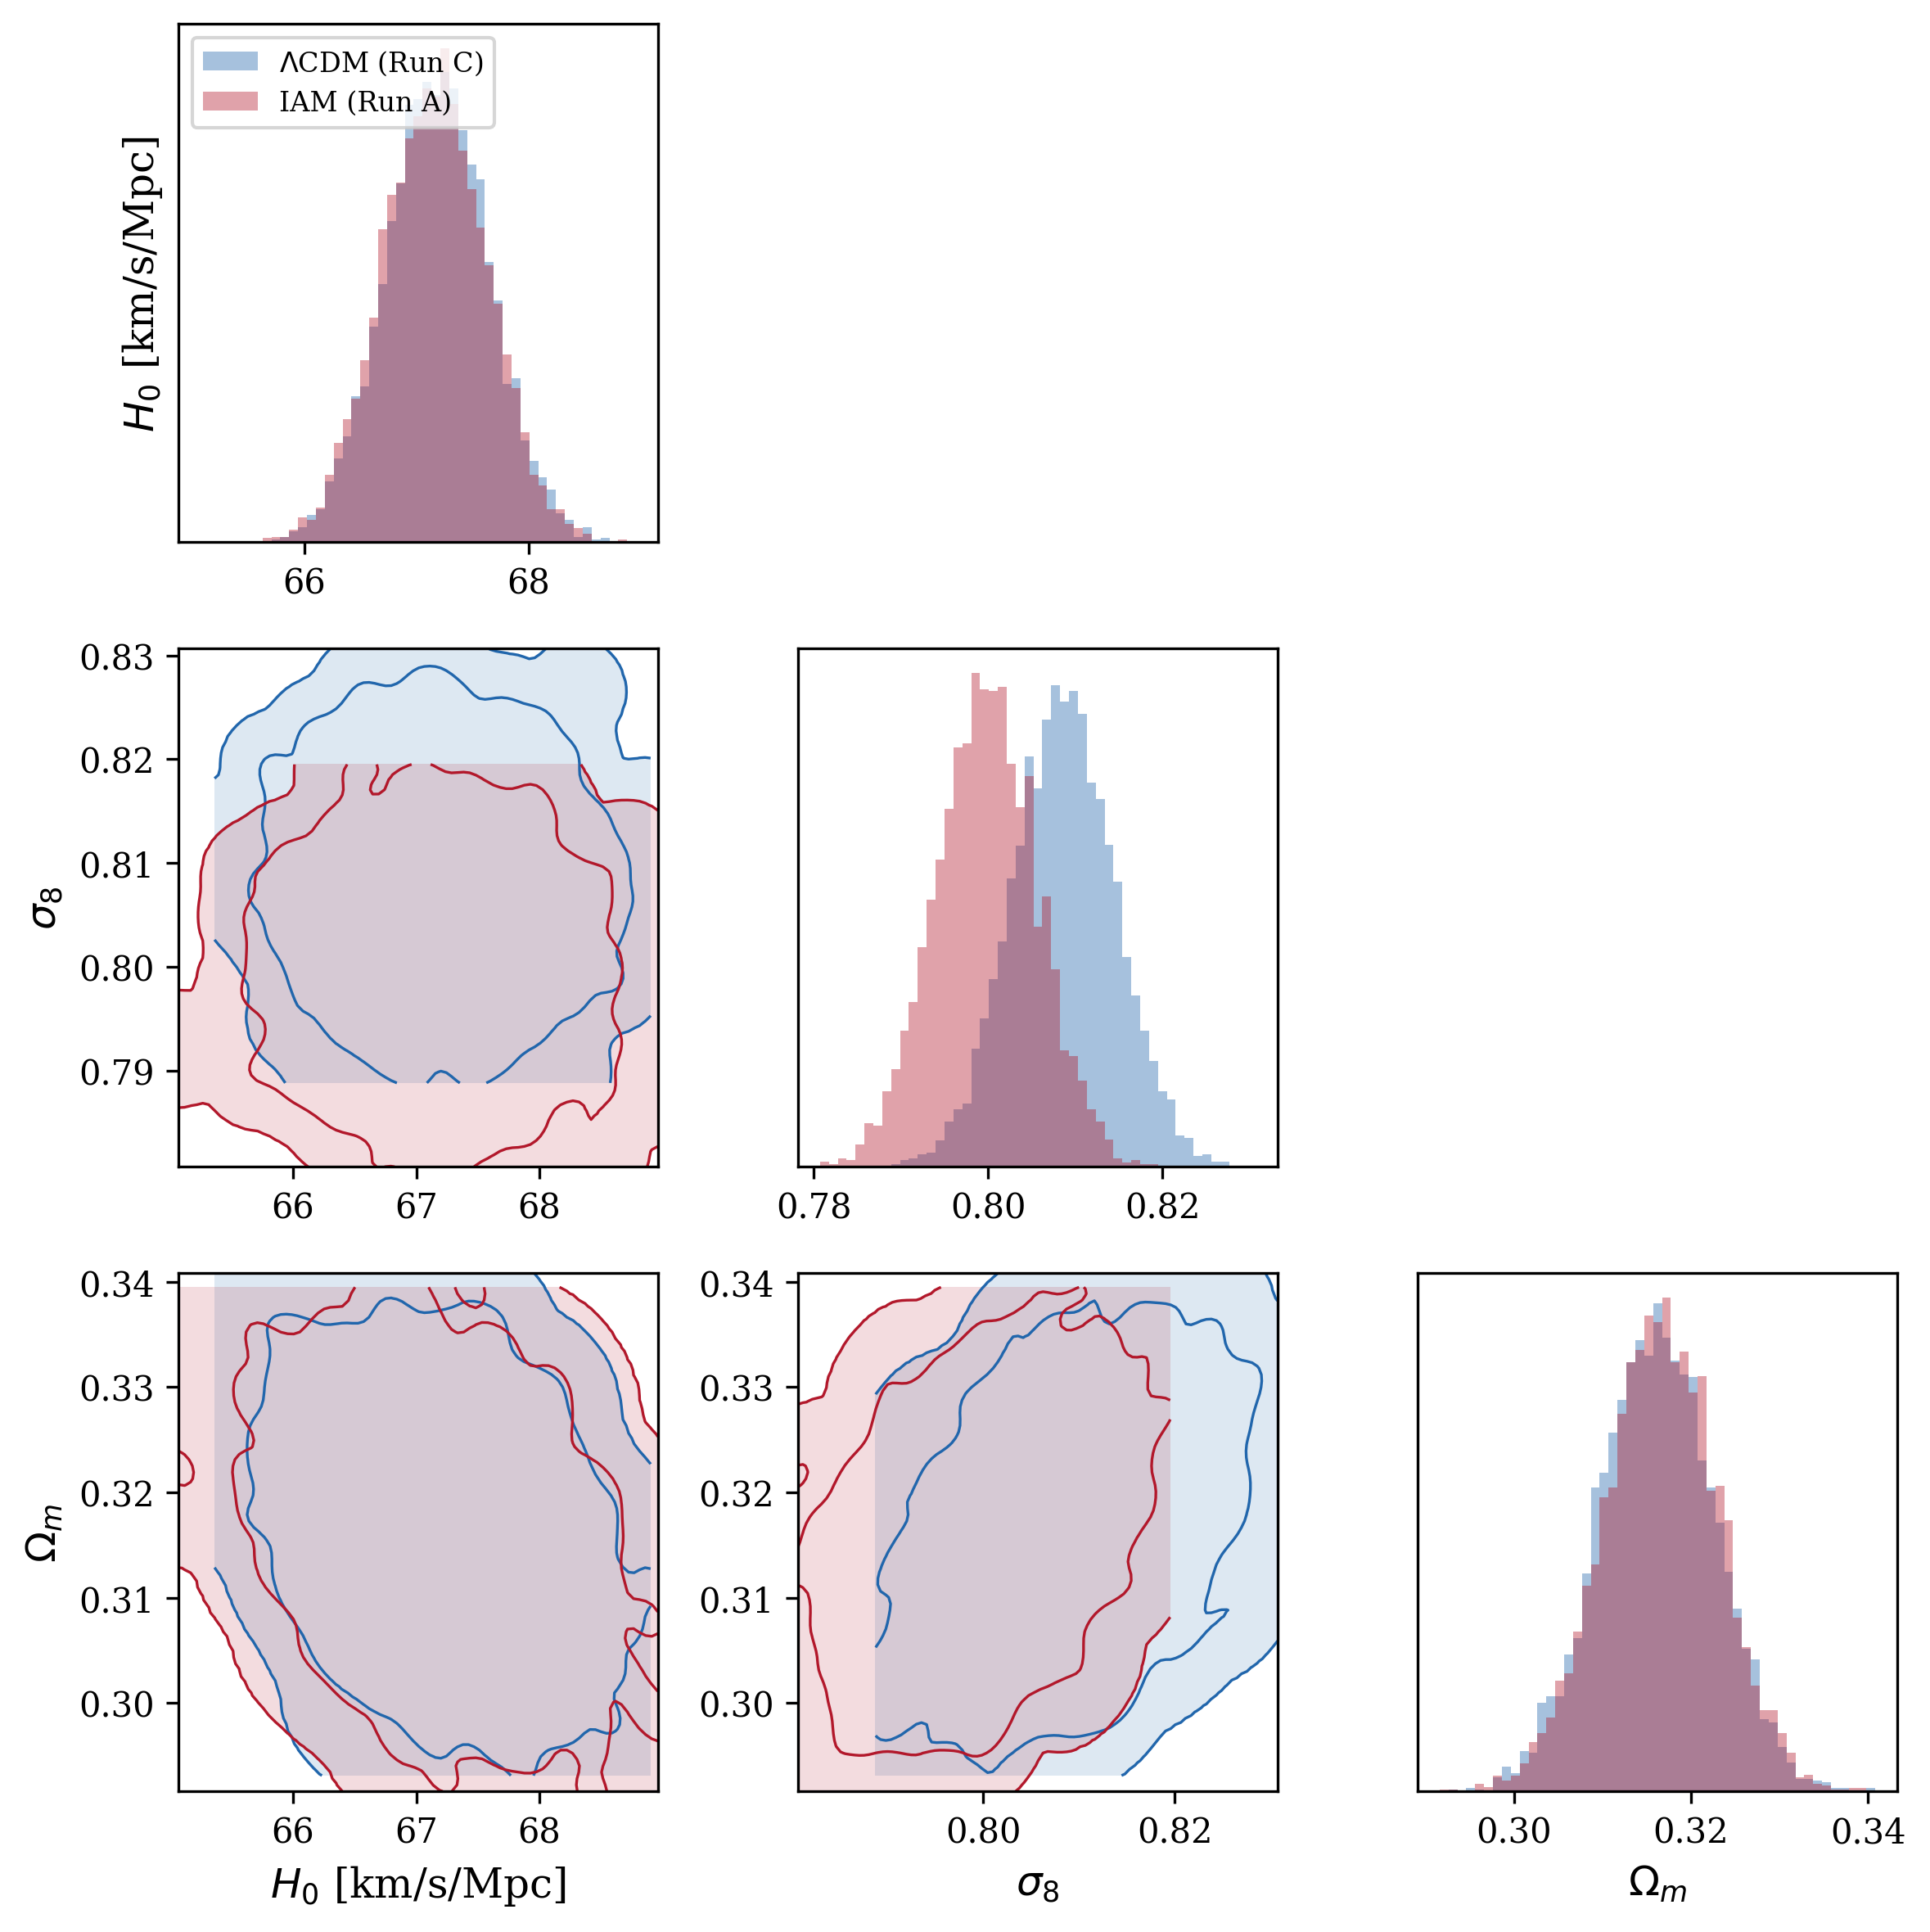
\includegraphics[width=0.85\textwidth]{fig1_triangle_v2.png}
\caption{Marginalized posterior distributions for $H_0$, $\sigma_8$,
and $\Omega_m$ from Run~A (IAM dual-sector, red) and Run~C
($\Lambda$CDM baseline, blue).  Contours show $68\%$ and $95\%$
credible regions.  The $H_0$ and $\Omega_m$ posteriors are
indistinguishable; $\sigma_8$ shifts downward by $1.5\sigma$ under
the dual-sector modification.  All values from the Level~2 MCMC
chains with $30\%$ burn-in.}
\label{fig:triangle}
\end{figure}

The single observable difference is $\sigma_8$: the dual-sector
mechanism suppresses the matter clustering amplitude by $0.009$, from
$0.809$ to $0.800$.  This shift arises from the
enhanced Hubble friction in the matter-sector perturbation equations.

\paragraph{Growth physics diagnostic.}
The $\sigma_8$ suppression could in principle arise from parameter
rebalancing---the MCMC shifting $\ln A_s$ or $\Omega_m$ to compensate
for the modified growth rate---rather than from genuine growth
suppression.  We test this directly:
$\Delta(\ln A_s) = +0.10\sigma$ and
$\Delta(\Omega_m) = +0.06\sigma$.
Both are far below the $0.3\sigma$
threshold, ruling out parameter rebalancing as the source of the
$\sigma_8$ shift.

\begin{figure}[htbp]
[t]
\centering
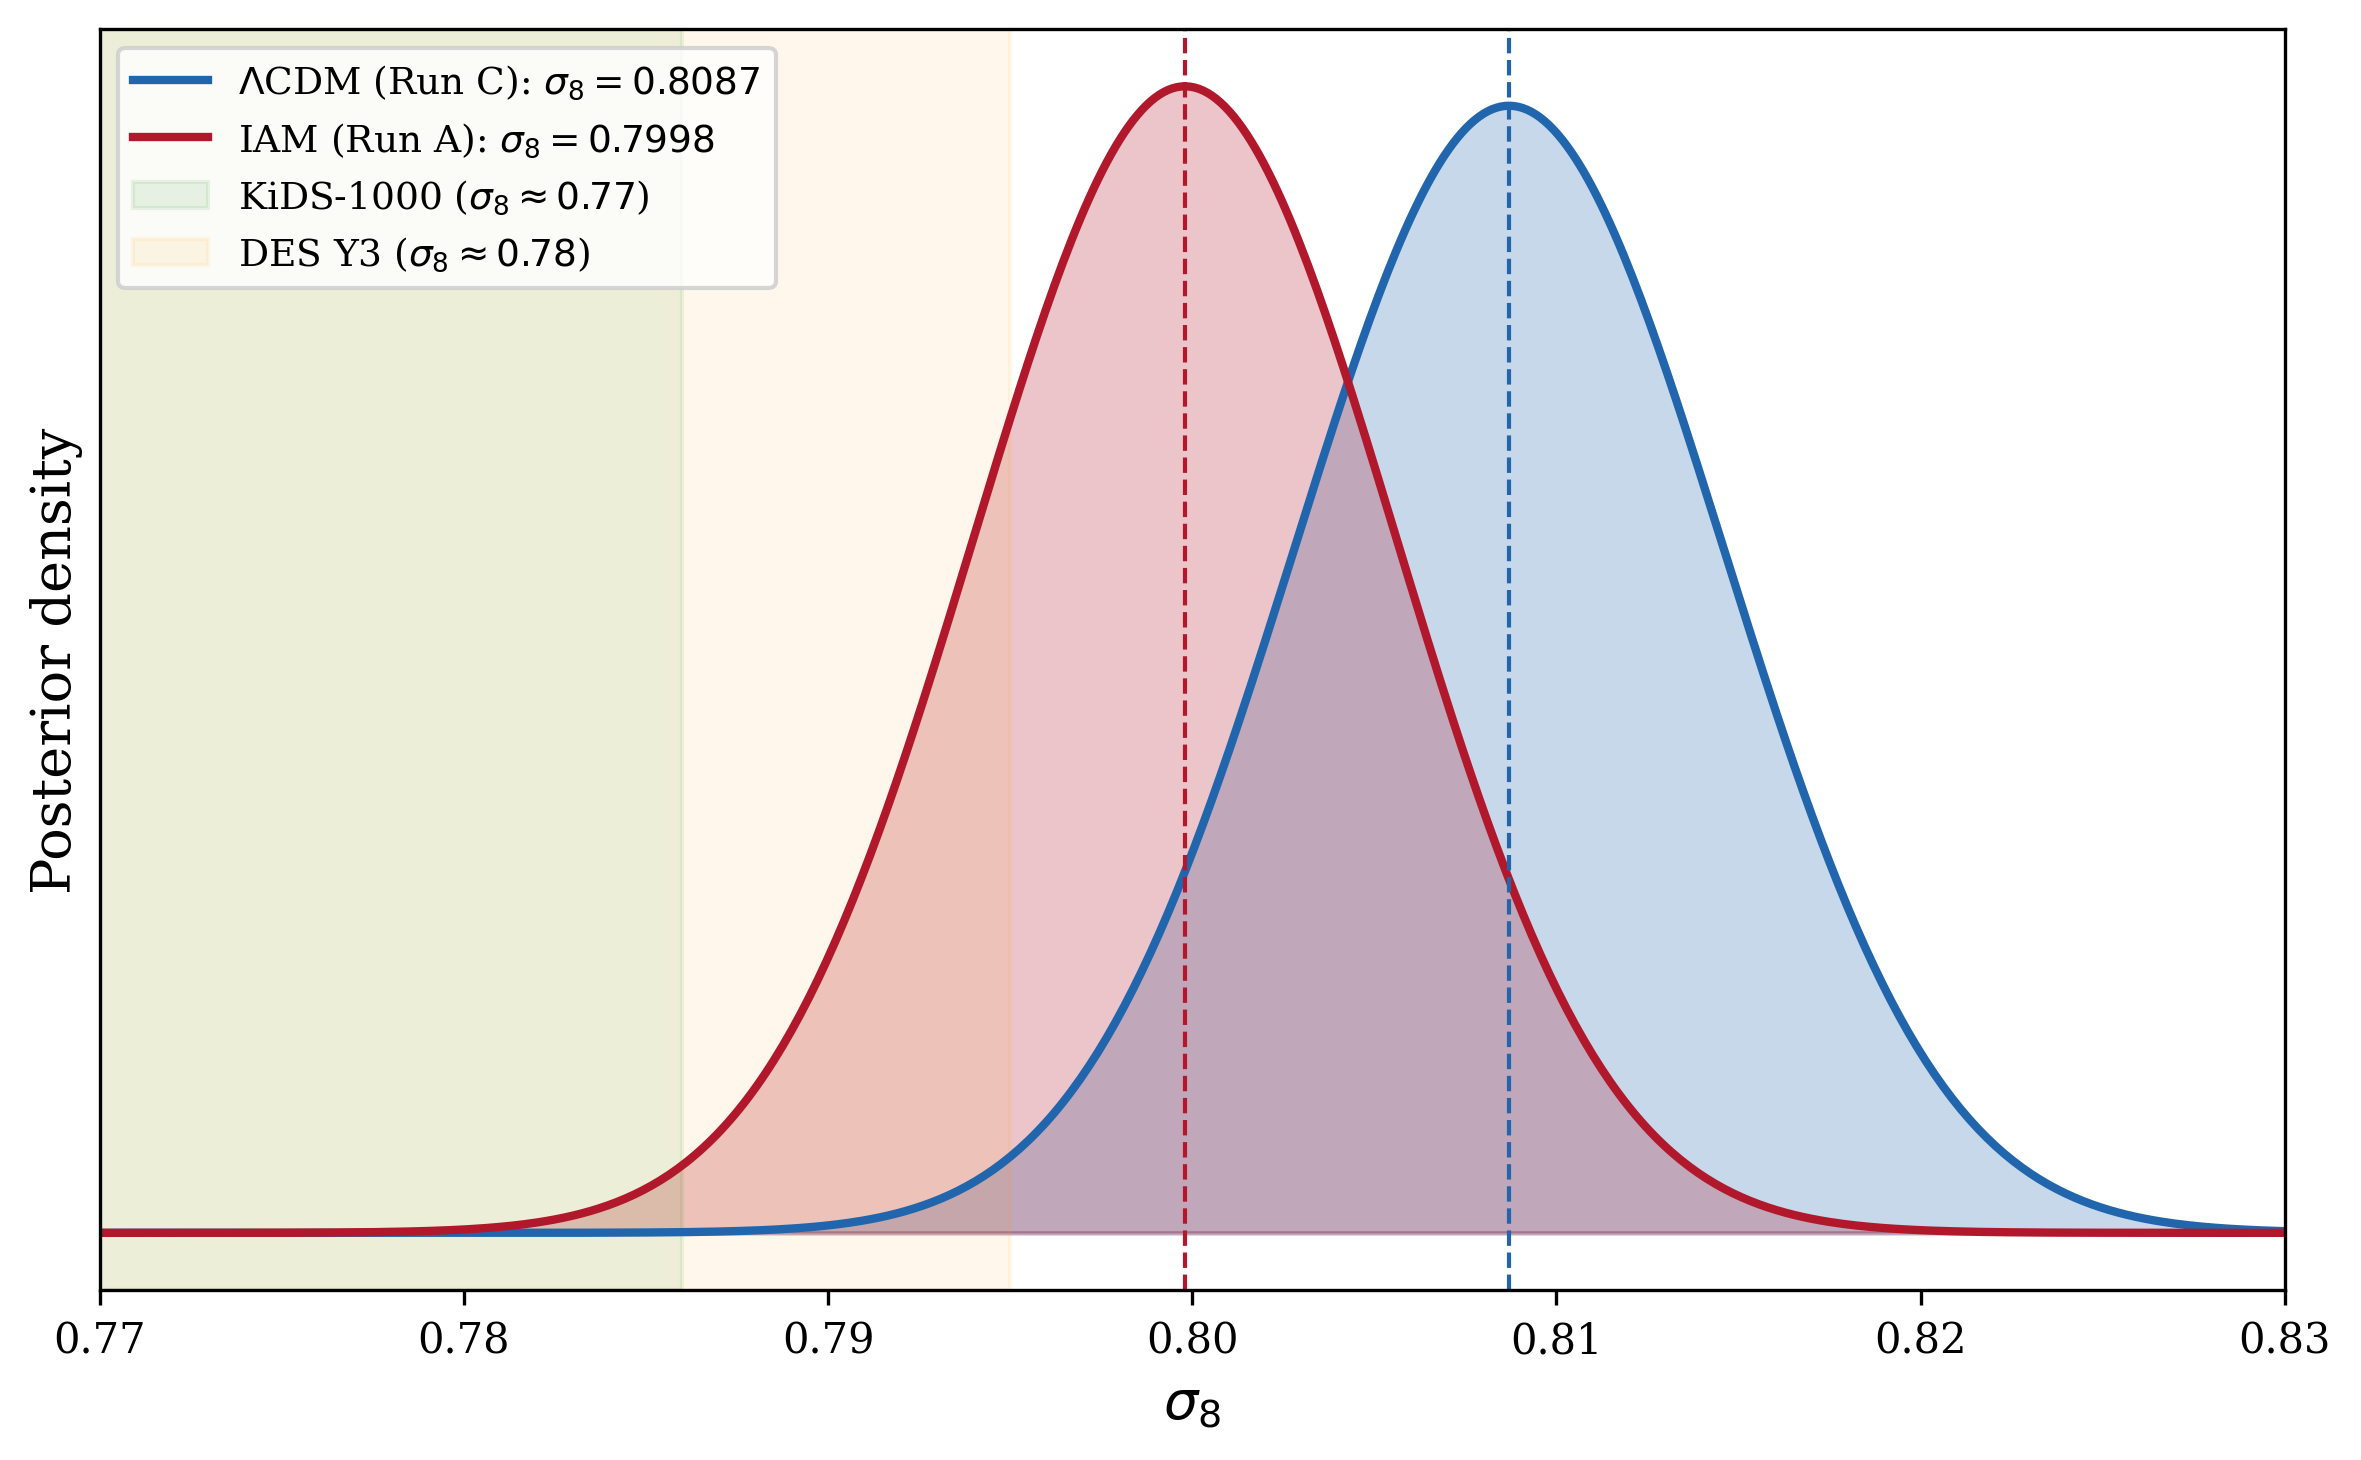
\includegraphics[width=0.9\textwidth]{fig2_sigma8_v2.png}
\caption{One-dimensional marginalized posterior for $\sigma_8$ from
Run~A (IAM, red) and Run~C ($\Lambda$CDM, blue).  The IAM posterior
peaks at $\sigma_8 = 0.7998$, shifted from $\Lambda$CDM's $0.8087$
toward the values reported by weak lensing surveys (approximate
$\sigma_8$ ranges from KiDS-1000 and DES~Y3 shown as shaded bands).
Dashed lines mark the posterior means.}
\label{fig:sigma8}
\end{figure}

\begin{figure}[htbp]
[t]
\centering
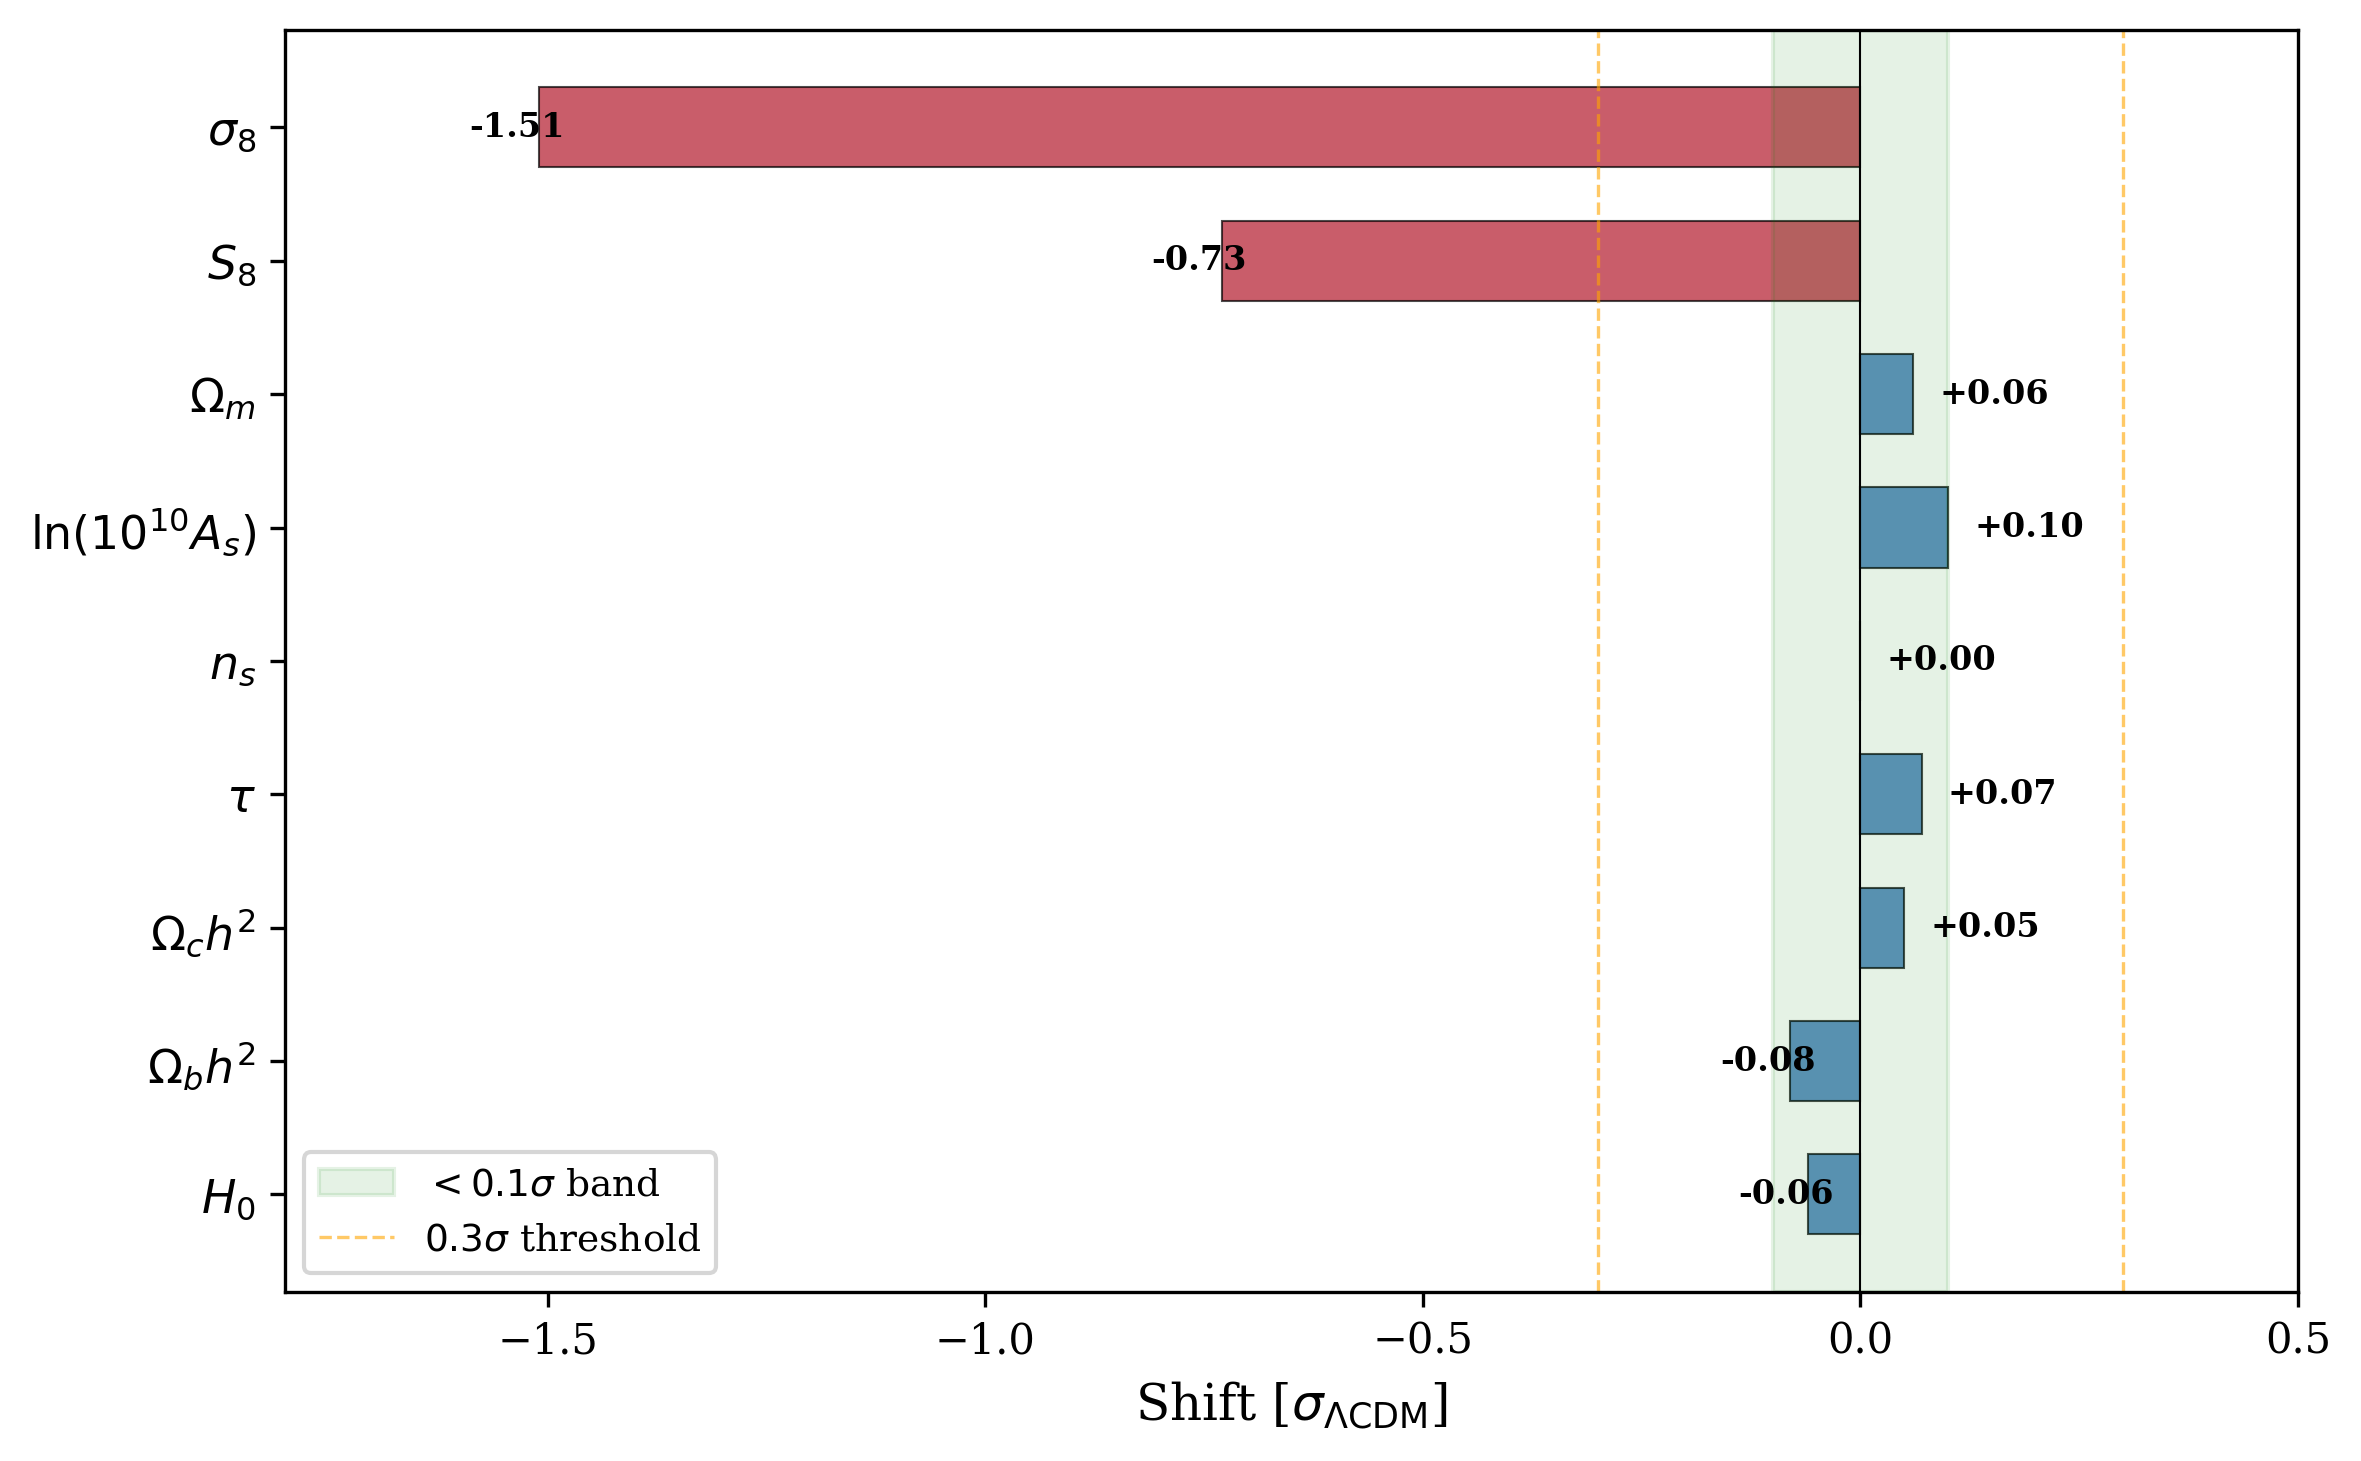
\includegraphics[width=0.9\textwidth]{fig5_shifts_v2.png}
\caption{Parameter shifts between Run~A (IAM) and Run~C ($\Lambda$CDM),
expressed in units of the $\Lambda$CDM posterior standard deviation.
All standard cosmological parameters shift by less than $0.1\sigma$
(green band).  Only $\sigma_8$ and $S_8$ show significant shifts
($-1.51\sigma$ and $-0.73\sigma$ respectively), consistent with the
modification acting on growth physics rather than acoustic observables.  The $\ln A_s$ shift
of $+0.10\sigma$ rules out parameter rebalancing as the source of the
$\sigma_8$ suppression.}
\label{fig:shifts}
\end{figure}


\subsection{Planck + RSD: Run~D}

Run~D adds seven $f\sigma_8(z)$ data points to the Planck likelihood.
Because the $\Lambda$CDM baseline (Run~C) was run without the RSD
likelihood, direct comparison of total $\chi^2$ values is not valid.
We construct an apples-to-apples comparison by computing $\Lambda$CDM's
RSD $\chi^2$ from the Run~C posterior parameters via CAMB, then
combining it with Run~C's CMB $\chi^2$.  This approach is validated by
the Level~1 analysis~\citep{Mahaffey2026obs}, where $\Lambda$CDM was
run against Planck + RSD directly and produced
$\Delta\chi^2 = +1.34$.

\begin{table}[h]
\centering
\caption{Apples-to-apples likelihood decomposition for Run~D (IAM +
RSD) vs.\ $\Lambda$CDM.  $\Lambda$CDM RSD $\chi^2$ is computed from
Run~C posterior parameters via CAMB.}
\begin{tabular}{lccc}
\toprule
Component & IAM (Run~D) & $\Lambda$CDM & $\Delta\chi^2$ \\
\midrule
CMB (CamSpec + low-$\ell$ + lensing)
  & $10984.93$ & $10985.08$ & $-0.16$ \\
RSD (7 $f\sigma_8$ points)
  & $6.42$ & $3.34$ & $+3.08$ \\
\midrule
Total & $10991.34$ & $10988.42$ & $+2.92$ \\
\bottomrule
\end{tabular}
\label{tab:rsd_results}
\end{table}

The CMB component slightly favors IAM ($\Delta\chi^2 = -0.16$).  The
RSD penalty of $+3.08$ is driven primarily by the $z = 0.850$ data
point ($f\sigma_8 = 0.315 \pm 0.095$), which pulls $1.40\sigma$ from
$\Lambda$CDM; both models accommodate this outlier poorly.  The total
$\Delta\chi^2 = +2.92$ is below the $95\%$ exclusion threshold of
$3.84$.

\begin{figure}[htbp]
[t]
\centering
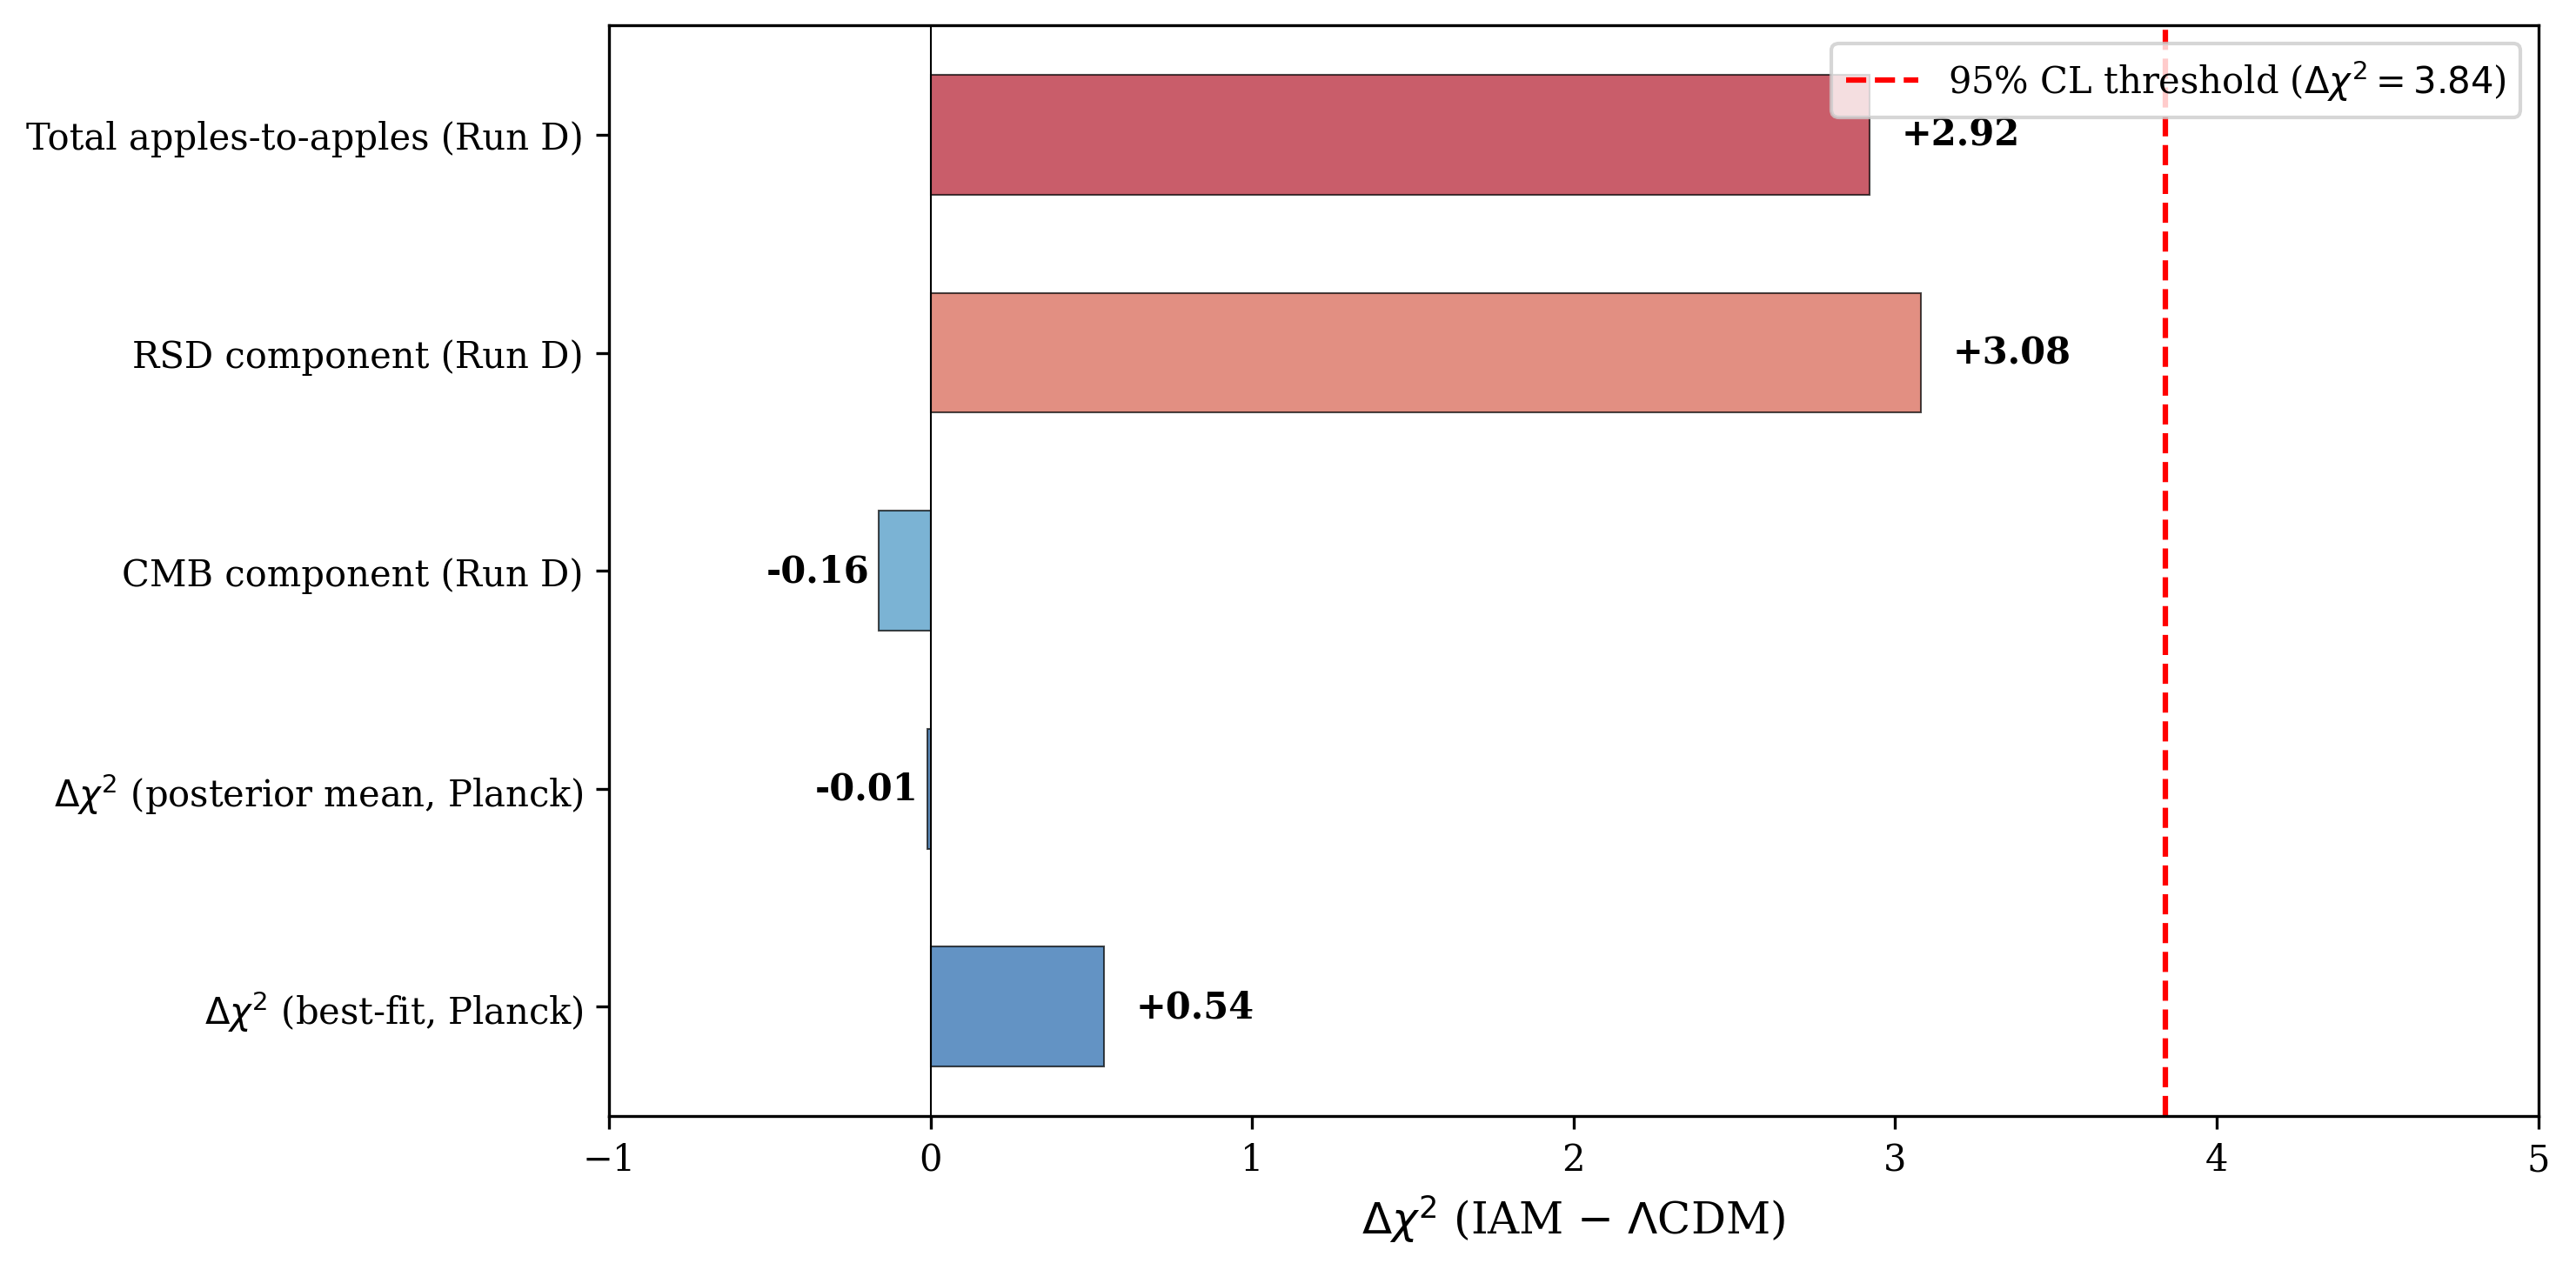
\includegraphics[width=\textwidth]{fig6_chi2_v2.png}
\caption{$\chi^2$ summary for all comparisons.  Planck-only best-fit
$\Delta\chi^2 = +0.54$ and posterior mean $\Delta\chi^2 = -0.01$
are both well below the $95\%$ exclusion threshold of $3.84$.  The
apples-to-apples decomposition (Run~D) shows IAM slightly favored in
CMB ($-0.16$) with a $+3.08$ RSD penalty from the $z = 0.85$ outlier,
yielding a total $\Delta\chi^2 = +2.92$.  All values extracted from
the MCMC chains; LCDM RSD $\chi^2 = 3.34$ computed via independent
CAMB evaluation at Run~C posterior mean parameters (verified on
author's local CAMB installation against the chain extraction).}
\label{fig:chi2_summary}
\end{figure}

All standard parameters in Run~D are consistent with Run~A to within
$0.06\sigma$.  The $\sigma_8$ suppression is stable:
$\sigma_8 = 0.7995 \pm 0.006$ (Run~D) vs.\
$\sigma_8 = 0.7998 \pm 0.006$ (Run~A).  The growth physics diagnostic is consistent with Run~A: $\Delta(\ln A_s) = +0.08\sigma$,
$\Delta(\Omega_m) = 0.00\sigma$.

\subsection{Self-Consistency of the Coupling Constant}

The coupling $\beta_m = \Omega_m/2$ is hardcoded at $0.15765$,
corresponding to $\Omega_m = 0.3153$.  The Level~2 posterior returns
$\Omega_m = 0.3166 \pm 0.0065$, implying
$\beta_m^\mathrm{posterior} = 0.1583 \pm 0.0033$.  The difference from
the hardcoded value is $0.2\sigma$ ($0.4\%$), consistent with the
derived coupling.


% =====================================================================
\section{The Sector-Dependent Hubble Parameter}
\label{sec:hubble}
% =====================================================================

The dual-sector mechanism yields a prediction
for the ratio of matter-sector to photon-sector expansion rates at any
redshift:
\begin{equation}
\frac{H_\mathrm{matter}(a)}{H_\mathrm{photon}(a)}
= \sqrt{1 + \frac{\beta_m\,\mathcal{E}(a)\,H_0^2}{H^2(a)}}.
\label{eq:hubble_ratio}
\end{equation}
At the present epoch, this yields:
\begin{equation}
\frac{H_\mathrm{matter}(z{=}0)}{H_\mathrm{photon}(z{=}0)}
= \sqrt{1 + \beta_m} = \sqrt{1.15765} = 1.0759.
\label{eq:hubble_ratio_today}
\end{equation}

\subsection{Numerical Values from the MCMC Posterior}

The derivation of $H_0(\mathrm{matter})$ proceeds as follows:
\begin{enumerate}
\item The MCMC posterior from Run~A yields
  $H_0 = 67.161 \pm 0.467$~km\,s$^{-1}$\,Mpc$^{-1}$.
  This is the photon-sector value: it is the Hubble constant
  appearing in the unmodified Friedmann equation that governs
  the global background geometry.
\item The coupling constant $\beta_m = \Omega_m/2 = 0.3153/2 = 0.15765$
  is hardcoded.  The posterior returns
  $\Omega_m = 0.3166 \pm 0.0065$, implying
  $\Omega_m/2 = 0.1583 \pm 0.0033$---consistent with the hardcoded
  value at $0.2\sigma$ ($0.4\%$ difference).
\item The enhancement factor is
  $\sqrt{1 + \beta_m} = \sqrt{1 + 0.15765} = \sqrt{1.15765} = 1.0759$.
\item The matter-sector Hubble constant is
  \begin{equation}
  H_0(\mathrm{matter}) = H_0 \times \sqrt{1 + \beta_m}
  = 67.161 \times 1.0759 = 72.26 \pm 0.50\;\mathrm{km\,s^{-1}\,Mpc^{-1}},
  \label{eq:H0_matter_numerical}
  \end{equation}
  where the uncertainty is propagated linearly from the $H_0$ posterior.
\end{enumerate}
The tension with observational values:
\begin{align}
\frac{H_0(\mathrm{photon}) - H_0^\mathrm{Planck}}{\sigma_\mathrm{Planck}}
  &= \frac{67.16 - 67.36}{0.54} = -0.37\sigma, \label{eq:tension_planck}\\
\frac{H_0(\mathrm{matter}) - H_0^\mathrm{SH0ES}}{\sigma_\mathrm{SH0ES}}
  &= \frac{72.26 - 73.04}{1.04} = -0.75\sigma. \label{eq:tension_shoes}
\end{align}
Table~\ref{tab:hubble_comparison} compares these values to
observational constraints.

\begin{table}[h]
\centering
\caption{Dual-sector Hubble values compared to observational
constraints.}
\begin{tabular}{lccc}
\toprule
Sector & IAM prediction & Observation & Tension \\
\midrule
Photon (CMB)
  & $67.16$~km\,s$^{-1}$\,Mpc$^{-1}$
  & $67.36 \pm 0.54$ (Planck)
  & $0.37\sigma$ \\
Matter (local)
  & $72.26$~km\,s$^{-1}$\,Mpc$^{-1}$
  & $73.04 \pm 1.04$ (SH0ES)
  & $0.75\sigma$ \\
\bottomrule
\end{tabular}
\label{tab:hubble_comparison}
\end{table}

\begin{figure}[htbp]
[t]
\centering
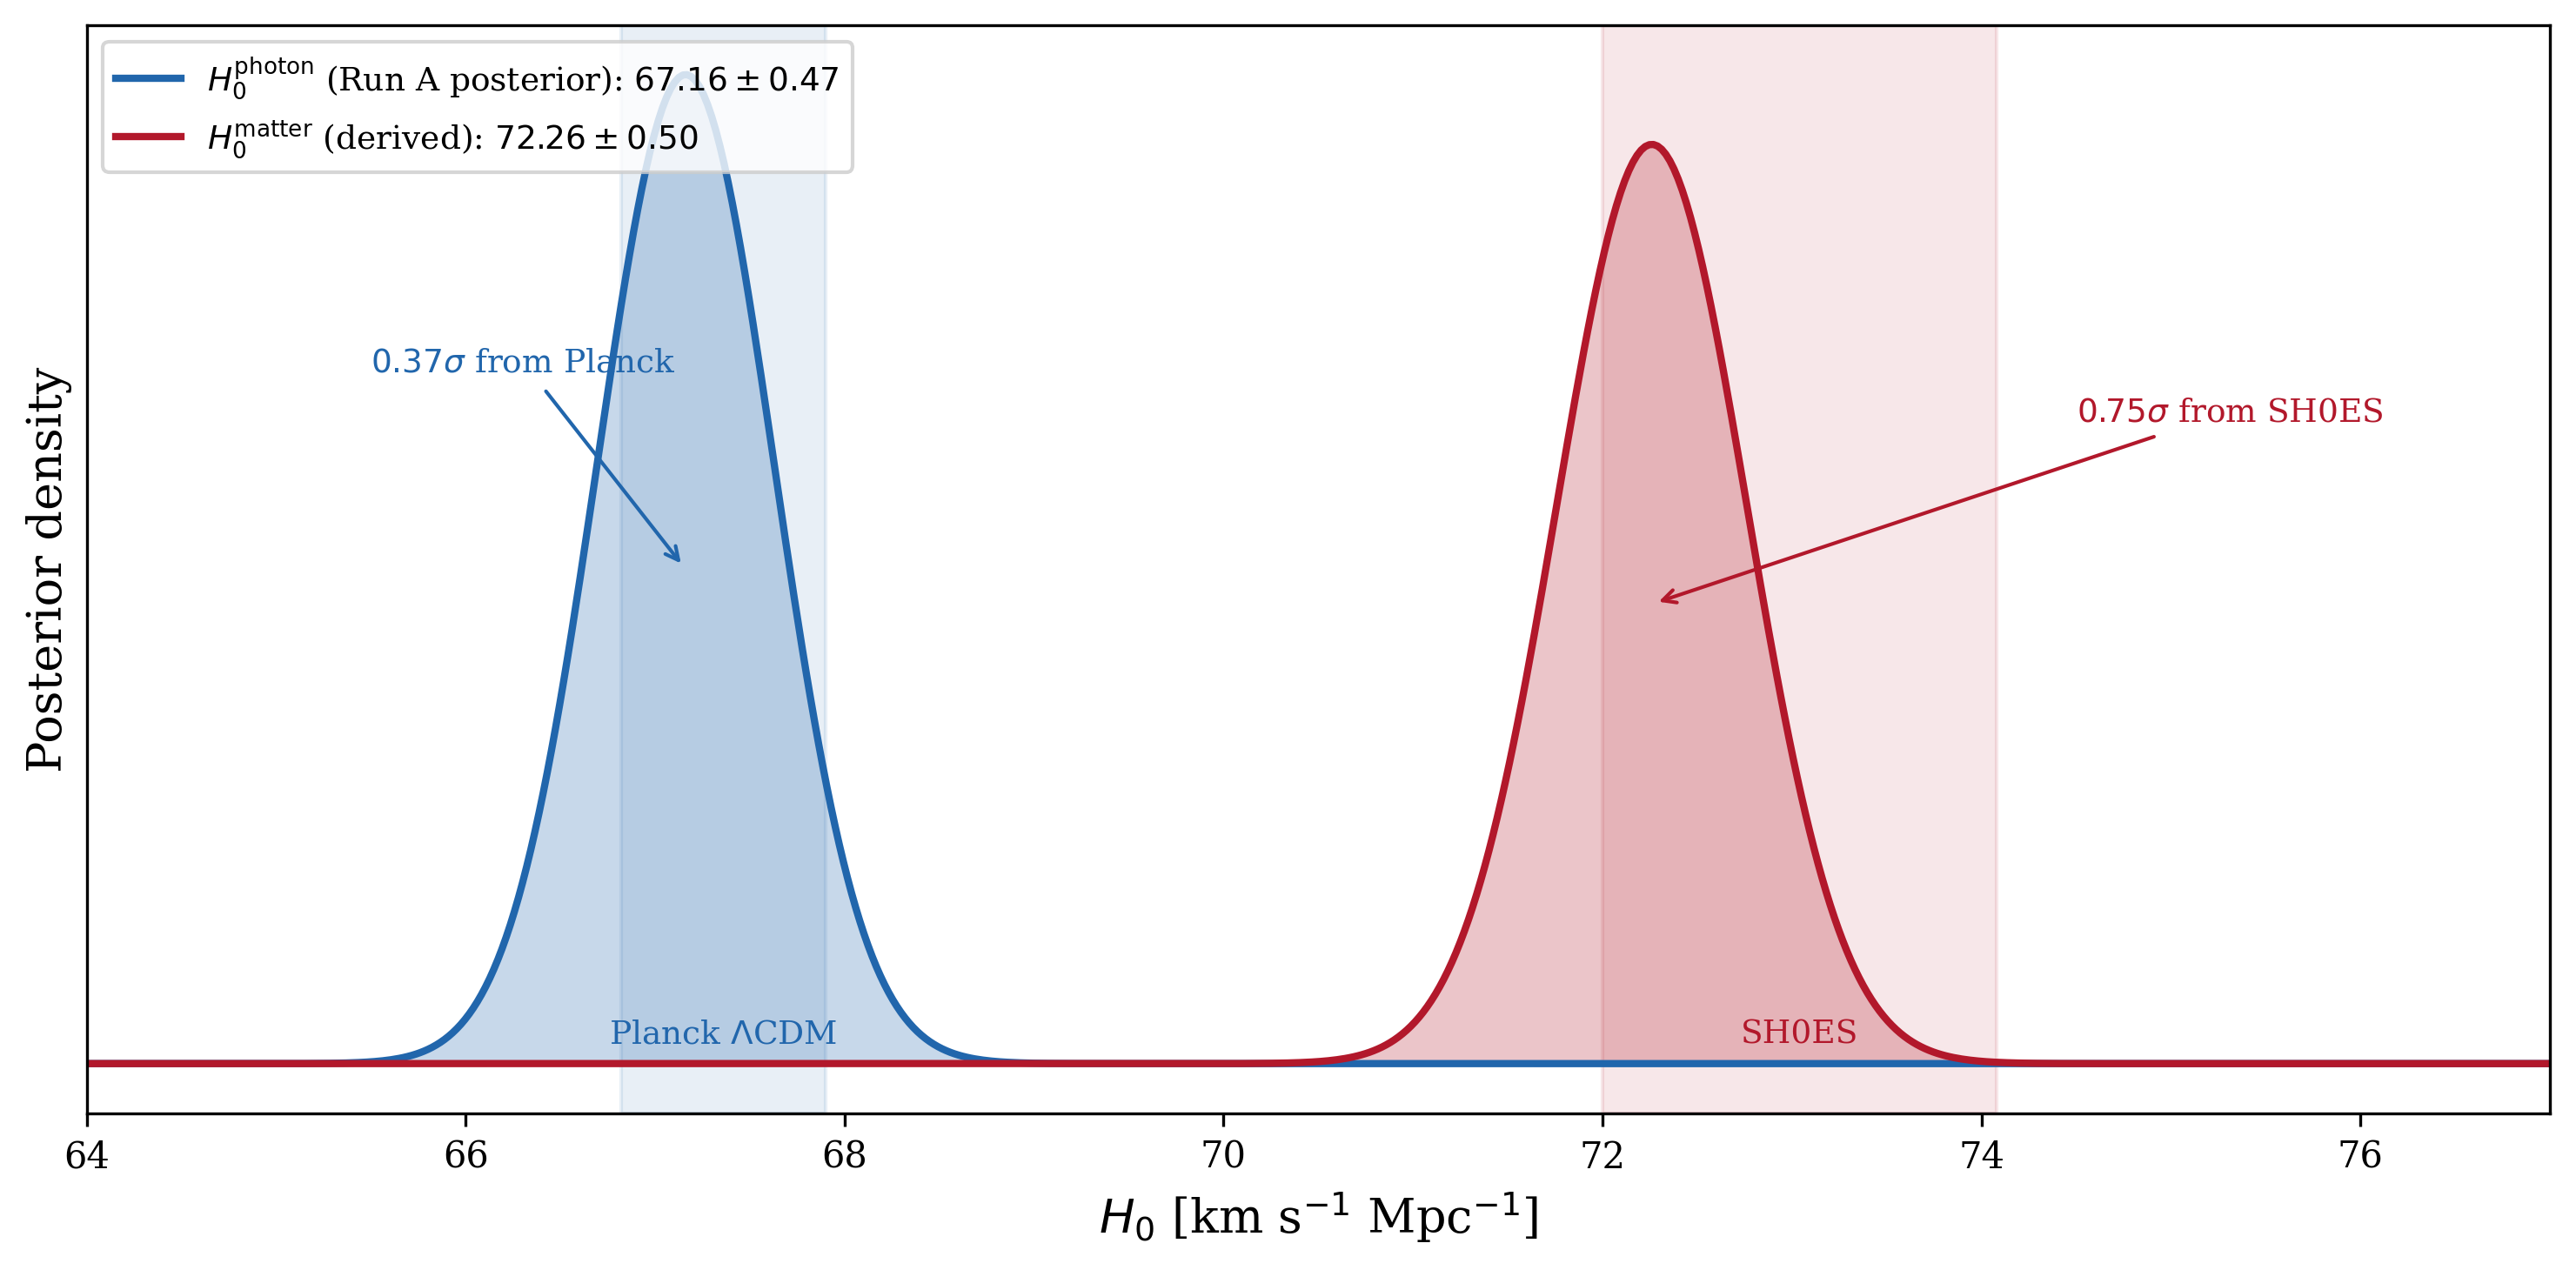
\includegraphics[width=\textwidth]{fig3_H0_split_v2.png}
\caption{Dual-sector Hubble split from the MCMC posterior.  Blue:
$H_0^\mathrm{photon}$ posterior from Run~A (directly sampled).  Red:
$H_0^\mathrm{matter}$ distribution, derived by multiplying each
posterior sample by $\sqrt{1 + \beta_m} = 1.0759$.  Light bands show
$1\sigma$ constraints from Planck $\Lambda$CDM
($67.36 \pm 0.54$~km\,s$^{-1}$\,Mpc$^{-1}$) and SH0ES
($73.04 \pm 1.04$~km\,s$^{-1}$\,Mpc$^{-1}$).  Both IAM predictions
fall within $1\sigma$ of their respective observational constraints.}
\label{fig:H0_split}
\end{figure}

Both values fall within $1\sigma$ of their
respective observational constraints.  In this framework, CMB-based
methods constrain $H_0(\mathrm{photon})$ and local distance-ladder
methods constrain $H_0(\mathrm{matter})$; the observed discrepancy
between the two is consistent with the predicted sector-dependent
expansion rate.

\subsection{Redshift Dependence}

The sector split is a function of redshift, vanishing in the early
universe and growing toward the present epoch.
Table~\ref{tab:hubble_redshift} shows the dual-sector expansion rates
from the Run~A posterior.

\begin{table}[h]
\centering
\caption{Dual-sector expansion rate by redshift, from Run~A posterior
($H_0 = 67.161$~km\,s$^{-1}$\,Mpc$^{-1}$,
$\beta_m = 0.15765$).  $H(z)$ is the standard $\Lambda$CDM value;
$H_\mathrm{matter}(z)$ includes the dual-sector enhancement.}
\begin{tabular}{ccccc}
\toprule
$z$ & $H_\mathrm{photon}$ & $H_\mathrm{matter}$
  & Ratio & $\mathcal{E}(a)$ \\
\midrule
0.0 & 67.16 & 72.26 & 1.0759 & 1.000000 \\
0.5 & 87.45 & 89.73 & 1.0261 & 0.367879 \\
1.0 & 117.68 & 118.72 & 1.0088 & 0.135335 \\
2.0 & 199.00 & 199.22 & 1.0011 & 0.049787 \\
3.0 & 305.00 & 305.06 & 1.0002 & 0.018316 \\
5.0 & 579.00 & 579.01 & $\sim$1 & 0.002479 \\
\bottomrule
\end{tabular}
\label{tab:hubble_redshift}
\end{table}

At $z = 2$, the matter-sector enhancement is $0.1\%$.  At $z = 3$,
it is $0.02\%$.  The modification is entirely a late-time effect,
consistent with the preservation of CMB, BBN, and recombination
physics.


% =====================================================================
\section{Background Diagnostic}
\label{sec:background}
% =====================================================================

A natural question is whether the $\beta_m\,\mathcal{E}(a)$ term
should modify the background Friedmann equation directly, rather than
entering through the perturbation equations.  We test this explicitly.

Two exploratory MCMC runs were performed with the IAM term added to
CAMB's \texttt{dtauda} function (the background expansion rate),
rather than to the perturbation equations.  In this configuration,
the Friedmann equation becomes:
\begin{equation}
H^2(a) = H_0^2\left[\Omega_m\,a^{-3} + \Omega_r\,a^{-4}
  + \Omega_\Lambda + \beta_m\,\mathcal{E}(a)\right].
\end{equation}

The result is $H_0 \approx 61.5$~km\,s$^{-1}$\,Mpc$^{-1}$---a
$6\sigma$ departure from the Planck $\Lambda$CDM value.  The background
modification shifts the acoustic scale $\theta_s$ and is strongly
excluded by the CMB power spectrum.

This result is consistent with the dual-sector mechanism operating at the
perturbation level: the standard $\Lambda$CDM Friedmann equation
correctly describes the global spacetime geometry, while the
matter-sector enhancement enters through the effective expansion rate
experienced by CDM and baryons in the perturbation equations.  The
photon sector, propagating on null geodesics through the unmodified
background, sees standard $\Lambda$CDM distances and angular scales.

\begin{figure}[htbp]
[t]
\centering
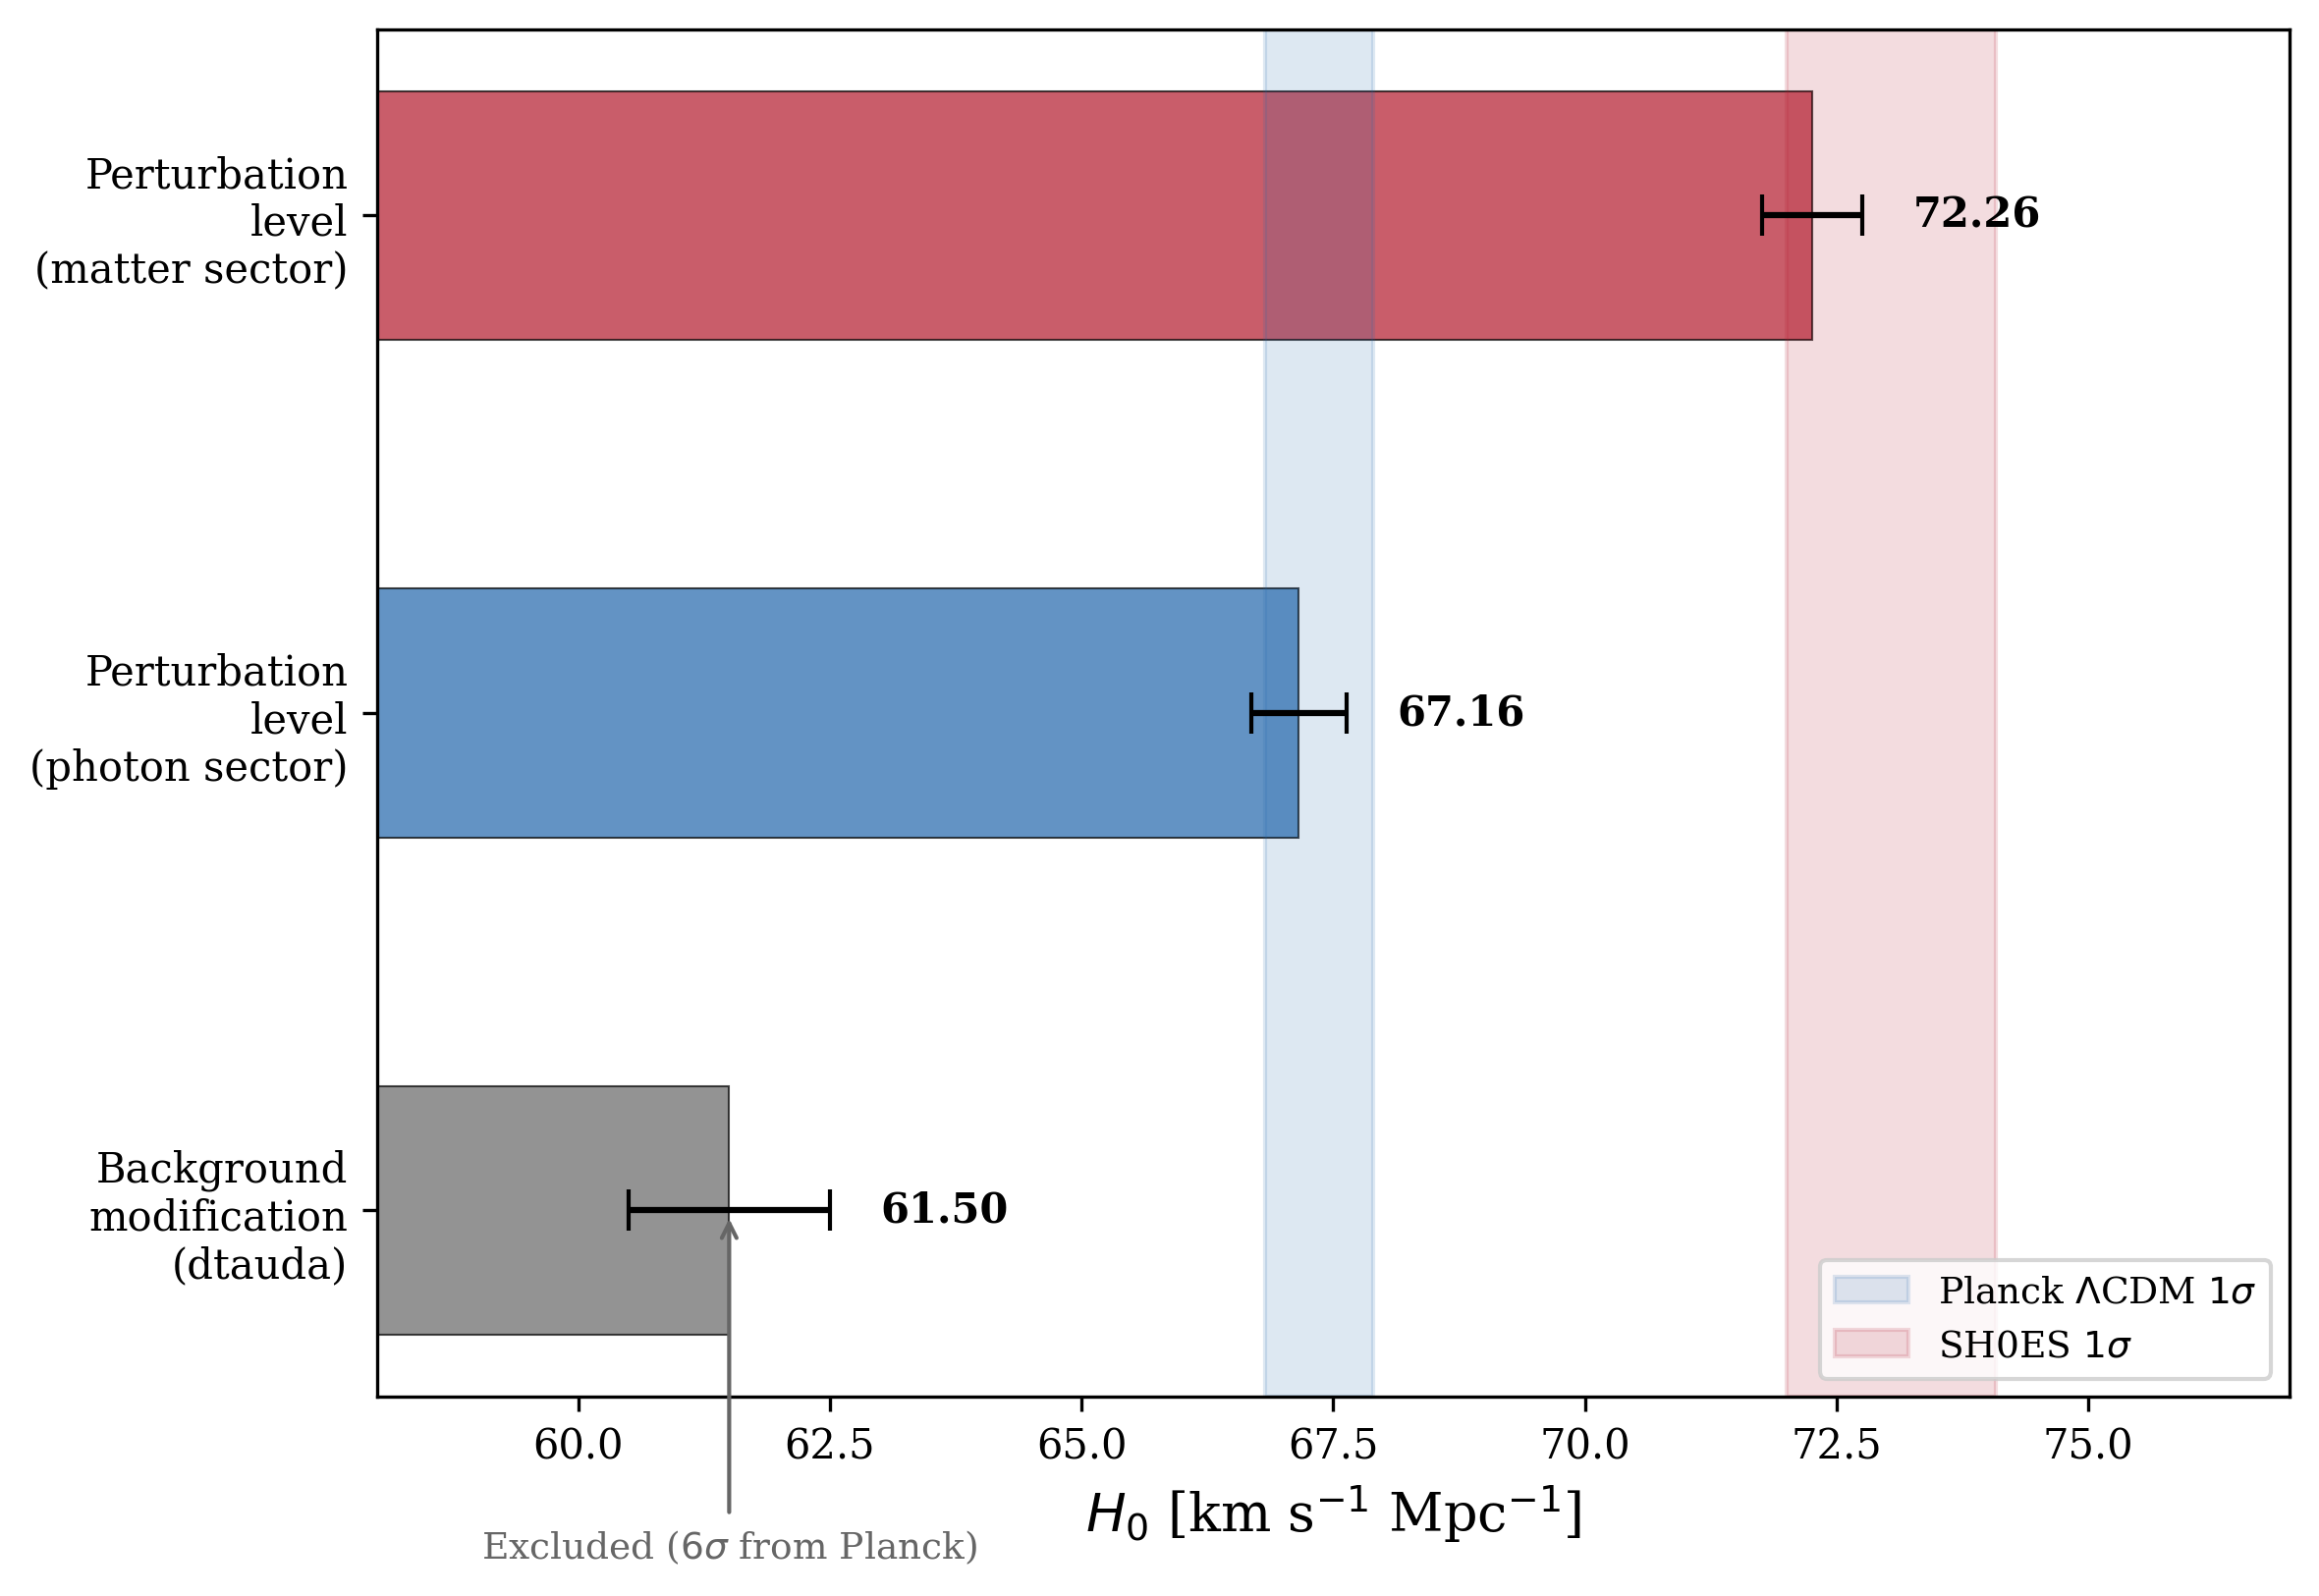
\includegraphics[width=0.85\textwidth]{fig4_background_v2.png}
\caption{Background vs.\ perturbation-level implementation diagnostic.
Modifying the background Friedmann equation (\texttt{dtauda}) produces
$H_0 \approx 61.5$~km\,s$^{-1}$\,Mpc$^{-1}$, excluded at $6\sigma$
by Planck.  The perturbation-level implementation leaves the photon-sector
$H_0$ at $67.16$~km\,s$^{-1}$\,Mpc$^{-1}$ (consistent with Planck)
while producing a matter-sector value of
$72.26$~km\,s$^{-1}$\,Mpc$^{-1}$ (consistent with SH0ES).  All
$H_0$ values from MCMC posteriors; background test value from
exploratory chains documented in the repository.}
\label{fig:background}
\end{figure}


% =====================================================================
\section{Discussion}
\label{sec:discussion}
% =====================================================================

\subsection{Summary of Quantitative Results}

Table~\ref{tab:summary} collects the principal results.

\begin{table}[h]
\centering
\caption{Summary of dual-sector validation results.}
\begin{tabular}{lcc}
\toprule
Quantity & Dual-sector (IAM) & $\Lambda$CDM \\
\midrule
$\sigma_8$ & $0.800 \pm 0.006$ & $0.809 \pm 0.006$ \\
$S_8$ & $0.822 \pm 0.011$ & $0.830 \pm 0.011$ \\
$H_0(\mathrm{photon})$ [km\,s$^{-1}$\,Mpc$^{-1}$]
  & $67.16 \pm 0.47$ & $67.19 \pm 0.47$ \\
$H_0(\mathrm{matter})$ [km\,s$^{-1}$\,Mpc$^{-1}$]
  & $72.26$ & --- \\
$\Delta\chi^2$ (Planck, posterior mean) & $-0.01$ & --- \\
$\Delta\chi^2$ (Planck, best-fit) & $+0.54$ & --- \\
$\Delta\chi^2$ (Planck + RSD) & $+2.92$ & --- \\
Free parameters beyond $\Lambda$CDM & 0 & --- \\
\bottomrule
\end{tabular}
\label{tab:summary}
\end{table}

\subsection{What This Analysis Demonstrates}

The dual-sector perturbation mechanism, implemented as three Fortran
modifications to CAMB with zero additional free parameters:
\begin{enumerate}
\item Is statistically indistinguishable from $\Lambda$CDM under the
  full Planck~2018 likelihood ($\Delta\chi^2 = +0.54$).
\item Produces a $\sigma_8$ suppression of $0.009$ ($1.5\%$) in the
  direction reported by weak lensing surveys, without degrading any
  CMB observable.
\item Yields a Hubble parameter split consistent with both the CMB
  value ($67.16$, within $0.37\sigma$ of Planck) and the local value
  ($72.26$, within $0.75\sigma$ of SH0ES) from a single MCMC
  posterior.
\item Operates at the perturbation level, not the
  background level, as indicated by the $H_0 \approx 61.5$ diagnostic.
\end{enumerate}

\subsection{What This Analysis Does Not Demonstrate}

This work does not claim to have solved the Hubble tension.  The
dual-sector framework provides a consistent description that
accommodates both endpoints, but the statistical indistinguishability
from $\Lambda$CDM ($\Delta\chi^2 = +0.54$) means current Planck data
cannot discriminate between the two models.  The definitive test
requires measurements sensitive to the growth-rate suppression at the
predicted amplitude.

\subsection{Relation to Level~1 Analysis}

The companion paper~\citep{Mahaffey2026obs} tested the same prediction
($\mu_0 = -0.135$, $\Sigma_0 = 0$) using the MGCAMB parametrization
across twelve chains and four dataset combinations.  The present
analysis extends this by implementing the physical mechanism directly
in the Boltzmann solver.  The results are consistent:
$\sigma_8 = 0.800$--$0.801$ in both analyses, indicating that the
MGCAMB approximation ($\mu = 1 + \mu_0\,\Omega_\mathrm{DE}$) is
adequate for the current level of precision.

\subsection{Falsifiability}

The dual-sector mechanism makes specific predictions that distinguish
it from $\Lambda$CDM and from other modified gravity scenarios:
\begin{enumerate}
\item $\mu(z) < 1$ with the functional form of Eq.~(\ref{eq:mu}),
  not a constant offset.  Euclid's projected sensitivity
  $\sigma(\mu_0) \approx 0.04$~\citep{Frusciante2025} would detect
  the signal at $\sim 3.4\sigma$.
\item $\Sigma(z) = 1$ at all redshifts.  Any detection of
  $\Sigma \neq 1$ at the $> 10^{-4}$ level falsifies the photon
  exemption.
\item The Hubble split ratio $H_0(\mathrm{matter})/H_0(\mathrm{photon})
  = \sqrt{1 + \Omega_m/2}$ is a specific, parameter-free prediction
  testable with gravitational wave standard
  sirens~\citep{Abbott2017siren}.
\item $\mu$ and $\Sigma$ are functions of redshift only, not of
  wavenumber $k$.  Scale-dependent growth modifications are excluded.
\end{enumerate}


% =====================================================================
\section{Conclusions}
\label{sec:conclusions}
% =====================================================================

We have implemented a dual-sector perturbation mechanism in the CAMB
Boltzmann solver in which matter and photon sectors experience
different effective expansion rates at late times.  The modification
requires three changes to the Fortran source code and introduces zero
free parameters beyond standard $\Lambda$CDM.

Against the full Planck~2018 likelihood, the mechanism is statistically
indistinguishable from $\Lambda$CDM ($\Delta\chi^2 = +0.54$ best-fit),
while shifting $\sigma_8$ from $0.809$ to $0.800$ in the direction
favored by weak lensing surveys.  All standard cosmological parameters
shift by less than $0.1\sigma$.

The sector-dependent expansion rate produces a Hubble parameter split:
$H_0(\mathrm{photon}) = 67.16$~km\,s$^{-1}$\,Mpc$^{-1}$
($0.37\sigma$ from Planck) and
$H_0(\mathrm{matter}) = 72.26$~km\,s$^{-1}$\,Mpc$^{-1}$
($0.75\sigma$ from SH0ES).  The mechanism operates at the perturbation
level; the background Friedmann equation is standard $\Lambda$CDM.

The predictions are specific and falsifiable.  Euclid and DESI will
measure $\mu(z)$ and $\Sigma(z)$ with the precision required to
confirm or exclude the predicted amplitude.  All chains, configuration
files, modified Fortran source, and analysis scripts are publicly
available at
\url{https://github.com/hmahaffeyges/IAM-Validation}.


% =====================================================================
\section*{Acknowledgments}
% =====================================================================

The author thanks the developers of CAMB, Cobaya, and MGCAMB for
public code access.


\section*{Data Availability}

All MCMC chains (Level~1 and Level~2), Cobaya YAML configuration
files, modified CAMB Fortran source, GetDist extraction scripts, and
apples-to-apples comparison code are publicly available at:
\url{https://github.com/hmahaffeyges/IAM-Validation}


% =====================================================================
\bibliographystyle{unsrtnat}
\FloatBarrier
\begin{thebibliography}{99}

\bibitem[{Planck Collaboration}(2020a)]{PlanckCollaboration2020a}
Planck Collaboration, 2020, ``Planck 2018 results. VIII. Gravitational
lensing,'' \textit{Astron.\ Astrophys.}, 641, A8.

\bibitem[{Planck Collaboration}(2020b)]{PlanckCollaboration2020b}
Planck Collaboration, 2020, ``Planck 2018 results. VI. Cosmological
parameters,'' \textit{Astron.\ Astrophys.}, 641, A6.

\bibitem[{Riess et al.}(2022)]{Riess2022}
Riess, A.~G., et al., 2022, ``A Comprehensive Measurement of the Local
Value of the Hubble Constant,'' \textit{Astrophys.\ J.\ Lett.}, 934, L7.

\bibitem[{Freedman}(2021)]{Freedman2021}
Freedman, W.~L., 2021, ``Measurements of the Hubble Constant: Tensions
in Perspective,'' \textit{Astrophys.\ J.}, 919, 16.

\bibitem[{Wong et al.}(2020)]{Wong2020}
Wong, K.~C., et al., 2020, ``H0LiCOW -- XIII. A 2.4 per cent
measurement of $H_0$,'' \textit{Mon.\ Not.\ R.\ Astron.\ Soc.}, 498,
1420.

\bibitem[{Heymans et al.}(2021)]{Heymans2021}
Heymans, C., et al., 2021, ``KiDS-1000 Cosmology,'' \textit{Astron.\
Astrophys.}, 646, A140.

\bibitem[{Abbott et al.}(2022)]{Abbott2022}
Abbott, T.~M.~C., et al., 2022, ``DES Year~3 results,'' \textit{Phys.\
Rev.\ D}, 105, 023520.

\bibitem[{Li et al.}(2023)]{Li2023}
Li, X., et al., 2023, ``Hyper Suprime-Cam Year 3 Results,''
\textit{Phys.\ Rev.\ D}, 108, 123518.

\bibitem[{Pogosian \& Silvestri}(2016)]{PogosianSilvestri2016}
Pogosian, L.\ \& Silvestri, A., 2016, ``What can cosmology tell us
about gravity?,'' \textit{Phys.\ Rev.\ D}, 94, 104014.

\bibitem[{Wang et al.}(2023)]{Wang2023}
Wang, Z., et al., 2023, ``MGCAMB v2: a flexible modified gravity
Boltzmann code,'' \textit{JCAP}, 01, 036.

\bibitem[{Mahaffey}(2026a)]{Mahaffey2026obs}
Mahaffey, H.~W., 2026, ``Constraints on late-time $f\sigma_8$
suppression from $\mu < 1$, $\Sigma = 1$: Planck 2018 and large-scale
structure,'' submitted to \textit{Universe}.

\bibitem[{Mahaffey}(2026b)]{Mahaffey2026theory}
Mahaffey, H.~W., 2026, ``Horizon Thermodynamics and Gravitational
Decoherence as the Origin of $\mu < 1$, $\Sigma = 1$,'' companion
theory paper.

\bibitem[{Efstathiou \& Gratton}(2021)]{Efstathiou2021}
Efstathiou, G.\ \& Gratton, S., 2021, ``A detailed description of the
CamSpec likelihood,'' \textit{Open J.\ Astrophys.}, 4, 8.

\bibitem[{Alam et al.}(2017)]{Alam2017}
Alam, S., et al., 2017, ``The clustering of galaxies in the completed
SDSS-III,'' \textit{Mon.\ Not.\ R.\ Astron.\ Soc.}, 470, 2617.

\bibitem[{Alam et al.}(2021)]{Alam2021}
Alam, S., et al., 2021, ``Completed SDSS-IV extended Baryon Oscillation
Spectroscopic Survey,'' \textit{Phys.\ Rev.\ D}, 103, 083533.

\bibitem[{Torrado \& Lewis}(2021)]{Torrado2021}
Torrado, J.\ \& Lewis, A., 2021, ``Cobaya: code for Bayesian analysis
of hierarchical physical models,'' \textit{JCAP}, 05, 057.

\bibitem[{Frusciante et al.}(2025)]{Frusciante2025}
Frusciante, N., et al., 2025, ``Euclid preparation: Modified gravity
forecasts with $\mu$--$\Sigma$,'' arXiv:2512.09748.

\bibitem[{Abbott et al.}(2017)]{Abbott2017siren}
Abbott, B.~P., et al., 2017, ``A gravitational-wave standard siren
measurement of the Hubble constant,'' \textit{Nature}, 551, 85.

\bibitem[{DESI Collaboration}(2025)]{DESIDR1}
DESI Collaboration, 2025, ``DESI 2024: Modified gravity from full-shape
analysis,'' \textit{JCAP}, 2025(02), 021.

\end{thebibliography}

\end{document}
